%TC: macro \marginfootnote [other]
%TC: envir SCfigure [] other
%TC: macrocount beginSCfigure [figure]
\documentclass[11pt,twoside]{report}
\usepackage{preamble}
\setcounter{chapter}{3}
\graphicspath{{../img/}}
\def\includebibliography{}

\externaldocument{background}
\externaldocument{morphometric-framework}

\begin{document}
\chapter{Local structure in the hard sphere liquid}
\epigraph{\textbf{hardball 1.1} \emph{informal} Uncompromising and ruthless methods or dealings.}{Oxford English Dictionary}
\label{chapter:morphometric-applications}
\todo{Check which version of dictionary.}

The majority of this chapter contains work published as Ref.\ \cite{RobinsonPRL2019}.
Later stuff is new.

\section{Introduction}

While mean-field theories provide insight into complex phenomena, physical accuracy is ensured only by a proper treatment of correlations.
For example, the simplest case of two-body correlations is at the foundation of predictive theories of the liquid state \cite{Hansen2013}, colloids, and complex plasmas \cite{LikosPR2001,Ivlev2012}.
%, and some forms of active matter \cite{Bechinger2016}.
In particular, the thermodynamics of simple liquids with solely pairwise interactions can be exactly expressed in terms of two-body correlations \cite{Hansen2013}.
However, to resolve these integrated quantities \emph{spatially} into structural motifs, and \emph{temporally} into specific dynamical events, one needs to calculate many-body correlations.
While such a many-body approach may often be neglected in normal liquids, long-standing challenges such as the dramatic dynamical changes occurring in supercooled liquids approaching their glass transition \cite{BerthierRMP2011,RoyallPR2015} and phase transitions such as crystal nucleation \cite{RussoSR2012} call for a many-body description.

In the case of supercooled liquids, theories based on pair correlations such as the standard mode-coupling framework \cite{goetze} fail to account for activated events thus predicting a spurious ergodicity breaking transition \cite{BrambillaPRL2009,HallettNC2018}.
Activated dynamics are often rationalised through collective (i.e.\ many-body) effects within contrasting thermodynamic and purely dynamic scenarios \cite{LubchenkoARPC2007,TarjusJPCM2005,BiroliPRL2006,JanssenPRL2015,SzamelPTEP2013,ChandlerARPC2010}.
These include exact mean-field results in high dimensions \cite{ParisiRMP2010,CharbonneauARCMP2017} whose relevance in finite-dimensional systems is hotly debated \cite{WyartPRL2017}.
A finite-dimensional theoretical description of many-body effects is therefore much needed.

However, many-body correlations are challenging to compute and typically combine both energetic and entropic contributions.
Physical insight can be gleaned by exploring the potential energy landscape of isolated clusters \cite{Wales2004,ArkusPRL2009}, but such methods are only exhaustive for small system sizes.
This limitation has been partly addressed by embedding clusters in a mean-field approximation of the surrounding liquid \cite{MossaJCP2003,MossaJNS2006}.
\todo{Describe Mossa and Tarjus approach in detail.}
Nonetheless, this approach neglects by construction the intra-cluster entropic contributions that may dominate in the supercooled regime of interest.
Furthermore, computer simulations, which naturally deliver full many-body correlations are limited in the range of dynamics they can access, hampering an approach to the glass transition, except for recent developments for certain models \cite{BerthierPRL2016}.

Here we place theoretical predictions of many-body local structure on a fundamentally more rigorous footing using inhomogeneous liquid state theory \cite{EvansAP1979}, which we reviewed in section \ref{sec:dft} and advanced in the chapter \ref{chapter:morphometric-framework}.
We model the many-body interactions between a local subsystem and the remaining liquid, directly accessing the many-body \textit{free} energy of local arrangements of particles.
This allows us to predict the populations of specific local structures in the bulk system across the entire liquid phase and beyond the dynamically accessible supercooled regime.
\todo{Make clear that in terms of glassy theories our approach does lean more towards a local structure point of view.}

\section{Many-body correlations and surface tension}

We conceptually separate the liquid into $n$ spatially adjacent particles and the remaining degrees of freedom, acting as a solvent, which we treat within the grand-canonical ensemble, as sketched in Fig.\ \ref{fig:system}(a).
The joint probability density for simultaneously finding $n$ identical particles embedded in $\mathbb{R}^d$ at positions $\vec{r}^n := \{\vec{r}_1, \dots, \vec{r}_n\}$ \todo{Move this definition to an earlier chapter} is proportional to the \emph{$n$-particle distribution function} $g^{(n)}(\vec{r}^n)$ \cite{Hansen2013}.
For a homogeneous system, this can be formally expressed in terms of the \emph{potential of mean force}, the reversible work required to insert the particles at $\vec{r}^n$:
\begin{equation}\label{eq:potential-mean-force}
  \begin{split}
    \phi^{(n)}(\vec{r}^n) &\equiv - k_B T \ln g^{(n)}(\vec{r}^n) \\
    &= U(\vec{r}^n) + \Delta \Omega(\vec{r}^n) - n\mu^{ex}.
  \end{split}
\end{equation}
We denote by $U$ the total potential energy of the $n$ interacting particles and by $\Delta\Omega := \Omega - \Omega_\textrm{hom}$ the difference between the grand potential of the homogeneous liquid $\Omega_\textrm{hom}$ (related to the total volume and pressure by the relation $\Omega_\textrm{hom} = -pV$) and the grand potential of the system including the $n$-particle inhomogeneity.
Finally, $k_B T$ and $\mu^{ex}$ are the thermal energy and the excess chemical potential (with respect to the ideal gas) of the homogeneous liquid respectively.

For systems with excluded volume interactions, we can divide the space into a local component $\mathcal{L} \subset \mathbb{R}^d$ of volume $V_\mathcal{L}$ inaccessible to solvent degrees of freedom and the remaining space $\mathcal{R} = \mathbb{R}^d \setminus \mathcal{L}$ filled by solvent (Fig. \ref{fig:system}).
The dividing surface $\partial\mathcal{L}$ separates these two components with surface area $A_{\partial\mathcal{L}}$, creating a surface tension $\gamma$.
The solvent contribution to Eq.\ \eqref{eq:potential-mean-force} is then \begin{equation}\label{eq:surface-tension}
  \Delta \Omega[\mathcal{L}] =
  p V_\mathcal{L} + \gamma[{\partial\mathcal{L}}] A_{\partial\mathcal{L}}.
\end{equation}
Note that the surface tension is not unique as only the total grand potential must be independent of the choice of $\partial\mathcal{L}$ and can even change its sign for some choices of dividing surface \cite{BrykPRE2003}.
For simplicity we will consider one-component liquids with particles of diameter $\sigma$.
Letting $B_R(\vec{r}_i)$ denote a ball of radius $R$ at site $\vec{r}_i$, we choose the \emph{solvent accessible surface} \cite{LeeJMB1971} as the dividing surface such that $\mathcal{L} = \cup_{i=1}^n B_\sigma(\vec{r}_i)$ (Fig.\ \ref{fig:system}).

Following Ref.\ \cite{KonigPRL2004} we assume $\Delta\Omega$ is translation and rotation invariant, continuous (with respect to the Hausdorff metric), and additive.
Hadwiger's characterisation theorem \cite{Hadwiger1957} then ensures the surface tension adopts the so-called \emph{morphometric} form
\begin{equation}\label{eq:morphometric-surface-tension}
  \gamma[\partial\mathcal{L}] =
  \gamma_\infty +
  \frac{\kappa \, C_{\partial\mathcal{L}} + \overline{\kappa} \, X_{\partial\mathcal{L}}}
       {A_{\partial\mathcal{L}}},
\end{equation}
with integrated mean and Gaussian curvatures $C_{\partial\mathcal{L}}$ and $X_{\partial\mathcal{L}}$, and $\gamma_\infty,\kappa,\overline{\kappa}$ as thermodynamic coefficients to be determined.
$\gamma_\infty$ is the surface tension at a planar wall (i.e.\ the familiar macroscopic surface tension), whilst $\kappa$ and $\overline{\kappa}$ are ``bending energies'' accounting for curvature corrections occurring at small length scales.
These values are system (and state point) dependent, but do not depend on the local geometry, making the linear form of Eq.\ \eqref{eq:morphometric-surface-tension} desirable for calculation.
While strictly an approximation, we motivate Eq.\ \eqref{eq:morphometric-surface-tension} from numerical studies where it has been found to be highly accurate below the freezing volume fraction in hard spheres \cite{RothPRL2006,LairdPRE2012,BlokhuisPRE2013,UrrutiaPRE2014,Hansen-GoosJCP2014}, and from the early success of scaled particle theories \cite{ReissJCP1959,ReissJCP1960}.

\begin{SCfigure}
  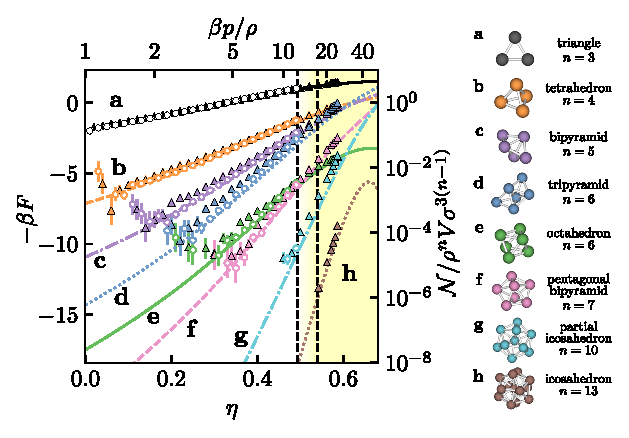
\includegraphics[width=\linewidth,center]{structure-populations}
  \caption[Concentration of local structures in the equilibrium liquid]{
    Static many-body structure in the hard sphere liquid: populations of small local structures in the hard sphere liquid determined from molecular dynamics simulations of 1372 monodisperse (open circles) and 8\% polydisperse (solid triangles) hard spheres against the theoretical prediction of this work (lines).
    Variations against volume fraction $\eta$ and compressibility $Z = \beta p/\rho$ shown.
    The hard sphere freezing and melting volume fractions are indicated by vertical dashed lines.
  }
  \label{fig:structure-populations}
\end{SCfigure}

\begin{SCfigure}
  \includegraphics[width=0.9\linewidth,outer]{n12-dos}
  \caption[Free energy distribution of 12 particle structures]{
    Theoretical free energy distribution for the $n=12$ local library of states at several volume fractions.
    The distribution is shifted to lower energies at higher volume fractions, and develops an increasingly bimodal structure.
    Populations are decomposed into those structures containing pentagonal bipyramids without octahedra (light fill) and the remaining structures (dark fill).
  }
  \label{fig:n12-dos}
\end{SCfigure}

\emph{Existing morphological theories.}---We focus on the hard sphere system because of its fundamental interest in the theory of liquids \cite{WidomS1967,Hansen2013}.
This allows suitable coefficients of Eq.\ \eqref{eq:morphometric-surface-tension} to be derived analytically by exploiting the geometric nature of hard spheres.
We compute morphological quantities and their derivatives following Ref.\ \cite{KleninJCC2011}, which we have extended to calculate curvature measures [see details in the Supplementary Material (SM)].
Note that hard spheres are athermal meaning density is the only control parameter and all free energies are really entropies; here we use ``supercooled'' to mean high density.

We assume the Carnahan-Starling (CS) equation of state \eqref{eq:cs-pressure} \cite{CarnahanJCP1969} because this pressure is used in the WBII theory and is accurate deep within the supercooled regime \cite{BerthierPRL2016} although it will fail at very large densities nearing random close packing.
The pair correlation produced by these coefficients is self-consistent with CS at contact by construction; moreover, the new coefficients provide a theory that outperforms the older WBII approach across the whole range of distances typical of neighbouring particles (SM).
This enables us to accurately model complex many-particle local structures.

\section{Free energy of local structures}

Owing to the high accuracy of the correlations produced with the new morphometric coefficients, we can now calculate many-body correlations in the supercooled regime.
We denote the population of some chosen local structure as $\mathcal{N} = \rho^n V \sigma^{3(n-1)} e^{-\beta F}$, where $F$ is the free energy of the local structure.
From the definition of $g^{(n)}$ as a probability distribution we write the free energy as
\begin{equation}\label{eq:local-structure-free-energy}
  \beta F = -\ln{
    \frac{1}{V \sigma^{3(n-1)}}
    \left(
    \int_{\mathcal{D}}
    g^{(n)}(\vec{r}^n) \, d\vec{r}^n
    \right)
  },
\end{equation}
where the domain of integration $\mathcal{D}$ \emph{defines} the local structure, and $g^{(n)}$ is calculated from the morphometric potential of mean force using Eqs.\ \eqref{eq:potential-mean-force}, \eqref{eq:surface-tension} and \eqref{eq:morphometric-surface-tension} (computational details in SM).
We define a particular local structure by its bond topology, using a pairwise cutoff $\sigma_{cut}$ such that separations between particles are in the range $r_{ij} \in [\sigma, \sigma_{cut}]$ if they are ``bonded'' and $r_{ij} > \sigma$ otherwise.
All results presented use a cutoff of $\sigma_{cut}=1.2 \sigma$, but we have tested our findings are are not significantly affected by a choice of $\sigma_{cut}=1.4 \sigma$ indicating their robustness.

To demonstrate the effectiveness of this approach we have taken rigid structures for $3 \le n \le 13$ which are global minima of clusters in simple liquids \cite{Wales2004}.
We determined their free energies at arbitrary volume fraction by thermodynamic integration (details in SM) of Eq.\ \eqref{eq:local-structure-free-energy}.
In the left panel of Fig.\ \ref{fig:structure-populations} we find excellent agreement between the theoretical prediction and the observed concentration of local structure seen in molecular dynamics simulations of both mono- and moderately polydisperse (8\%) hard spheres at all volume fractions accessed by the simulations i.e.\ $\eta \lesssim 0.585$ (details in SM).

Our approach is able to predict populations of local structures well beyond the regime dynamically accessible to simulation, finding nontrivial structural change deep in the glassy regime highlighted by a rescaling with respect to the trivial $\rho^n$ density contribution.
The free energy of considered structures changes approximately linearly across the entire liquid regime, with deviations from linear becoming more apparent in the supercooled regime.

All structures apart from the fourfold symmetric octahedron in Fig.\ \ref{fig:structure-populations} are subunits of the icosahedron, and increase in concentration more rapidly than the octahedron until high density.
For $n=6$ we consider the free energies of two structures: the tripyramid and octahedron.
We find that the tripyramid occurs $\sim20$ times more often than the octahedron, their free energy difference being dominated by the different point group symmetries following \cite{MalinsJPCM2009,MengS2010}.
We can also estimate vibrational contributions, which allow us to match not only the relative but also the absolute values of free energies obtained from simulation.
In particular, we are able to capture the gradual reduction of the population of octahedral motifs in favour of the tripyramids at high volume fractions.
This is related to the previously observed emergence of fivefold symmetric motifs (such as the full and partial icosahedron) \cite{RoyallPR2015,TarjusJPCM2005,HallettNC2018,DunleavyNC2015}, which is here directly predicted from liquid state theory.

Having tested that the theory is accurate for selected geometries, we now take the exhaustive list of 11980 rigid structures for $n=12$ determined in Ref.\ \cite{Holmes-CerfonSR2016} to obtain a local density of states for a given sized inhomogeneity.
These rigid structures correspond to unique contact topologies, but in thermal systems (i.e. with finite gaps between particles) we expect many of them to be indistinguishable as found in Ref.\ \cite{TrombachPRE2018}.
Nevertheless, because of their exhaustiveness these represent a complete local density of states in the liquid, of fundamental interest to random first-order transition theory \cite{LubchenkoARPC2007}.
We calculated the free energy of all (first-order) rigid (nonsingular) structures using Eq.\ \eqref{eq:local-structure-free-energy} (right panel of Fig.\ \ref{fig:structure-populations}), finding a bimodal distribution with two main peaks separated by a free energy difference that increases with increasing volume fraction.
We find the that lower energy distribution consists of structures rich in fivefold (icosahedral) symmetry in the absence of fourfold (octahedral) symmetry.

\begin{SCfigure}
  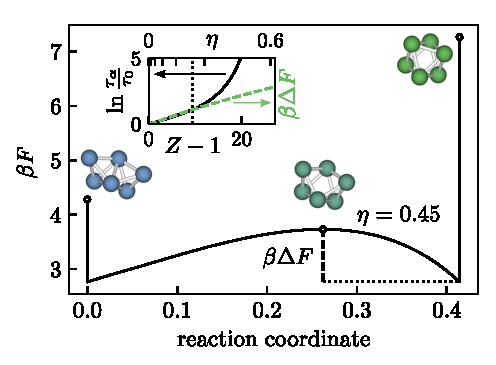
\includegraphics[width=0.9\linewidth,outer]{n6-reaction-path}
  \caption[The simplest nontrivial reaction path in hard spheres: octahedron to tripyramid]{
    Reaction for transition between tripyramid and octahedron $n = 6$ structures.
    Stationary points are indicated by markers: there is a discontinuity in free energy at the end points due to the additional integration over the reaction coordinate, and symmetry in the case of the octahedron.
    Inset: variation of activation barrier with volume fraction $\eta$ and compressibility $Z = \beta p/\rho$ from this theoretical reaction path (dashed line) and measured $\alpha$-relaxation times in bulk molecular dynamics simulations (solid line), where $\eta = 0.45$ is indicated with a vertical dotted line.
  }
  \label{fig:reaction-path-6}
\end{SCfigure}
\todo{Change compressibility factor to pressure}

\todo{Pictures of packings up to n7}

\section{Dynamics: free energy along a reaction path}

We have thus far focused on static thermodynamic properties: yet a connection with dynamics can be made by calculating the free energy along reaction paths between (geometrically similar) structures.
This calculation along unstable directions in the free energy landscape requires an analytic approach (described in the SM), and generates paths such as the one in Fig.\ \ref{fig:reaction-path-6}.
Here we consider transitions between the tripyramid and the octahedron with $n=6$ because this is the simplest nontrivial transition between distinct hard sphere packings (SM).
Comparing this dynamical barrier to the structural relaxation for ($\alpha$-) relaxation timescale $\tau_\alpha$ extracted from simulations relative to a microscopic time $\tau_0$ (inset of Fig.\ \ref{fig:reaction-path-6}), we find this single reaction path barrier agrees with the low density scaling of $\tau_\alpha$ (linear in the compressibility factor $\beta p / \rho$ \cite{BerthierPRE2009}).
However, activated dynamics are not expected in this regime so this agreement may be coincidental.
%Moving to high densities, hard spheres exhibit two-step relaxation when vibrational ($\beta$--) and full ($\alpha$--) relaxations decouple as the system approaches its glass transition \cite{Berthier2011}.
%However, dynamics along the tripyramid--octahedron path continues to increase in an ``Arrhenius'' fashion quite unlike the super-Arrhenius increase exhibited by the $\alpha$--relaxation in the computer simulations (inset of Fig.\ \ref{fig:reaction}).
%It has been shown in molecular systems that $\beta$--relaxation can be Arrhenius in the deeply supercooled regime where $\alpha$-- relaxation is super-Arrhenius \cite{Yu2015}.
%Given that typical particle displacements in the tripyramid--octahedron path are around 0.15$\sigma$ per particle, we observe that this relaxation mechanism may be more characteristic of ($\beta$--) relaxation than full ($\alpha$--) relaxation.
It is possible to extend our methodology for larger rearrangements, which may be sufficient to access ($\alpha$-) relaxation \emph{at very deep supercooling} for equilibrium systems.
However, the rapid growth in the number of possible states presents a considerable numerical challenge requiring new methods and approximations, so we leave this exciting avenue for future study.

\section{Conclusions}

We have presented a formalism for describing many-body correlations in liquids and developed it into an accurate and computationally efficient parameter-free theory for hard spheres using integral geometry relying solely on the choice of the equation of state.
The key approximations involved treating the grand potential as continuous and additive (related to extensivity), and imposing the correct contact value of $g^{(2)}(r)$.

We applied the framework to a selection of local structural correlations, therefore predicting nontrivial changes in the energy landscape with supercooling putting previous empirical observations on more solid ground.
In particular, our analysis provides evidence for the existence of two populations of structures with distinct symmetries and free energies which causes the local density of states to become increasingly bimodal at high densities.
We note that we have treated densities corresponding to a degree of supercooling only accessible using novel swap Monte Carlo techniques \cite{BerthierPRL2016}; however, these simulations introduce large polydispersity, changing the local structure \cite{CoslovichJPCM2018} and thus limiting direct comparison with our calculations for the monodisperse liquid.

Our framework can be easily adapted to more complex liquids such as systems with soft repulsive interactions and polydisperse mixtures \cite{KodamaJCP2011}.
Integral geometry underlies the core equation \eqref{eq:morphometric-surface-tension}, so this approach can extend to hard particles of more complex shapes where the interaction potential is still geometric in nature.
It is applicable to a more general class of liquids where the soft part of the potential may be treated as a perturbation around a hard core \cite{Hansen2013} such that a geometric decomposition still applies.
This suggests a new route for predicting static properties of equilibrium liquids, with direct applications to self-assembly, nucleation and protein structure.

\section{New notes.}

We wish to describe local structure.
Ultimately, we wish to learn about the structure of the energy landscape in hard spheres.
To do so we must characterise the main features of the landscape, namely the different geometric packings and assign weights (free energies) to them.
This is a worthy goal in its own right, perhaps not that interesting for hard spheres but useful for wider applications (e.g.\ predicting self assembly, guiding chemical synthesis, understanding protein folding kinetics and predicting the native state and design).

The path we take is as follows:
\begin{enumerate}
\item We need some means of weighting points in the energy landscape: we do this using the morphometric approach (cf previous chapter)
\item A means of characterising and approximating the entire phase space: energy landscape formalism (next). This has two subgoals:
  \begin{enumerate}
  \item Divide the landscape into stationary points: minima and saddles.
    These stationary points characterise submanifolds of the entire landscape, \emph{basins} in the case of minima and \emph{reaction paths} in the case of saddles.
  \item Integrate over connected manifolds with weight function (potential of mean force) to obtain their free energies.
  \end{enumerate}
\end{enumerate}

%Another way of saying this is we need an integrand and boundary conditions.

\subsection{Connection with energy landscape descriptions}

\begin{itemize}
  \item First describe the energy landscape description.
  \item Based on low-temperature expansion arguments.
  \item Mean-field: Laplace method/saddle-point.
  \item Gaussian expansion around this result (called Harmonic approximation in energy landscape/chemistry literature).
\end{itemize}

\begin{SCfigure}[H]
  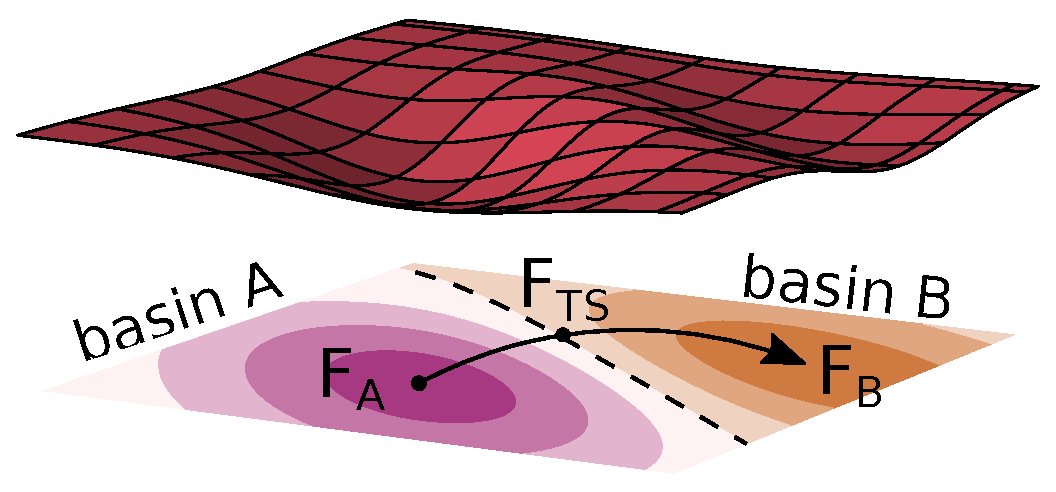
\includegraphics[width=\linewidth,outer]{toy-landscape}
  \caption[A cartoon energy landscape]{A cartoon energy landscape for a 2-dimensional phase space.
    The landscape features two local minima: $A$ and $B$.
    The area surrounding each minima defines its basin: any point from which the minima can be found by moving downhill belongs to the basin.
    Energy landscape approach: at low temperatures the system is expected to oscillate around potential energy minima, so the dynamics can be understood as rare events causing a change of basin.
    Thus a decomposition of the phase space in terms of basins should become exact for the dynamics at low temperatures in the supercooled regime of interest.}
\end{SCfigure}

In the case of local arrangements of hard spheres, rigid packings seem to correspond to minima of the potential of mean force.
I cannot prove this for the case of morphometric approach, but I cannot find a counter example.
Possibly can prove they are minimal volume.

\section{Locally favoured structures in hard spheres}

\subsection{Concentrations of local structure}

How do we define a local structure?
Most of the literature on structure in amorphous systems falls into one of either two categories
Almost all methods for Common methods:
\begin{itemize}
  \item Bond orientational order parameters
  \item Bond networks: take some bond detection algorithm (voronoi, 
Fom the partition function of the potential of mean force
Suppose we have a definition of a
\end{itemize}

From the definition of the probability density function in Eq.\ \eqref{eq:n-density-pdf}, the total number of local structures of a particular type in a volume $V$ is
\begin{equation}\label{eq:structure-population}
  \mathcal{N} =
  \int_{\mathcal{Q}} \rho^n g^{(n)}(\vec{r}^n) \, d\vec{r}^n,
\end{equation}
where $\mathcal{Q}$ is the domain \emph{defining} the local structure.
To get the free energy expression used in the main text we consider the manifold diffeomorphic to translations, defining $\mathcal{Q} = \mathcal{D} \rtimes \mathbb{V}$ where $\mathbb{V}\subset \mathbb{R}^3$ is the system volume.
Exploiting translational invariance of the potential of mean force, we fix one particle at the origin and integrate the center of mass over the system volume giving
\begin{equation}
  \mathcal{N} =
  \rho^n V \int_{\mathcal{D}} g^{(n)}(\vec{r}^n) \, d\vec{r}^{n-1}.
\end{equation}
We defined a free energy by taking $\mathcal{N} = \sigma^{3(n-1)} \rho^n V e^{-\beta F}$, which together with the above expression gives Eq.\ \eqref{eq:local-structure-free-energy} in the main text.

More generally, we consider the manifold diffeomorphic to translations \emph{and} rotations.
We define $\mathcal{Q} = \mathcal{D}' \rtimes SE(3)$ where $\textrm{SE}(d)$ is the $d$-dimensional special Euclidean group, leaving the $\mathcal{D}'$ as the space of the structure's internal motion.
\todo{Make this consistent with the notation of background chapter.}
We separate rigid body from internal motion by applying the following transformation to each particle coordinate
\begin{equation}
  \vec{r}(\{\vec{t}, \vec{\theta}, \vec{x}\}) =
  \vec{t} + \vec{R}(\vec{\theta}) \cdot \vec{q}(\vec{x}),
\end{equation}
where $\vec{t}$ is the translation vector, $\vec{\theta}$ the Euler angles, $\vec{R}$ the rotation matrix, and $\vec{x} \in \mathbb{R}^{3n-6}$ represents the internal coordinates.
We need to compute the metric of this transformation $G_{ij} = \vec{G}_i \vec{G}_i^T$ where the (generally curvilinear) basis vectors are $\vec{G}_i = \partial_i \vec{r}$.
To simplify calculation we choose $\vec{q}(\vec{x})$ to always be in the center-of-mass frame and orthogonal to rotations such that $G_{ij}$ reduces to block-diagonal form.
If the rotation matrix is expressed in Euler-angle representation as $\vec{R}(\vec{\theta}) = \vec{R}_3(\theta_3) \vec{R}_2(\theta_2) \vec{R}_1(\theta_1)$ then we have%
\marginfootnote{There is no elegent omitted step to obtain the form of $\vec{U}$ which gives the block diagonal form; rather, I used a series of educated guesswork within Mathematica to obtain this.
  There is probably a more direct route.}
\begin{equation}
  \vec{G}(\vec{\theta}, \vec{x}) =
  \begin{pmatrix}
    n \vec{E} & 0 & 0 \\
    0 & \vec{U}^T(\vec{\theta}) \vec{I}(\vec{x}) \vec{U}(\vec{\theta}) & 0 \\
    0 & 0 & \overline{\vec{G}}(\vec{x})
  \end{pmatrix},
\end{equation}
where $\vec{E}$ is the identity matrix, $\overline{\vec{G}}$ is the metric for internal motion, and we have defined the matrix $\vec{U}$ as
\begin{equation}
  \vec{U}(\vec{\theta}) =
  \begin{pmatrix}
    1 &  0              & -\sin{\theta_2} \\
    0 &  \cos{\theta_1} &  \cos{\theta_2} \sin{\theta_1} \\
    0 & -\sin{\theta_1} &  \cos{\theta_2} \cos{\theta_1} \\
  \end{pmatrix}
  \qquad
  \begin{aligned}
    \theta_1 &\in [0,2\pi] \\
    \theta_2 &\in \left[-\frac{\pi}{2},\frac{\pi}{2}\right] \\
    \theta_3 &\in [0,2\pi].
  \end{aligned}
\end{equation}
Note $\det{\vec{U}} = \cos{\theta_2}$.
The volume element in the new coordinates is
\begin{equation}
  d\vec{r}^n = \frac{\sqrt{\det G_{ij}(\vec{x})}}{\nu}
  \, d^3 \vec{t} \, d^3 \vec{\theta} \, d^{3n-6} \vec{x},
\end{equation}
where $\nu$ is the symmetry number (discussed below) and
\begin{equation}
  \sqrt{\det G_{ij}(\vec{x})} =
  \cos{\theta_2} \sqrt{\det{\vec{I}(\vec{x})}}
  \sqrt{n^3 \det{\overline{G_{ij}}(\vec{x})}}.
\end{equation}
The symmetry number emerges as the choice of internal coordinates typically fixes the particle labels breaking permutation symmetry; we have to multiply by the $n!$ possible labellings, which introduces double counting if the structure possesses rotational symmetry so we have to divide by the correcting factor $\nu$.
This is explained in detail in Ref.\ \cite{CatesSM2015}.
Thus \eqref{eq:structure-population} reduces to
\begin{equation}\label{eq:structural-partition-function-detailed}
  \frac{\mathcal{N}}{\rho^n V}
  =
  \frac{8\pi^2 \sqrt{n^3}}{\nu} \int_{D'}
  g^{(n)}(\vec{x}) \,
  \sqrt{\det{\overline{G_{ij}}(\vec{x})} \det{\vec{I}(\vec{x})}}
  \, d^{3n-6} \vec{x}.
\end{equation}
Note that in the limit of linear molecules, i.e.\ where all particles fall on a line, the above approach fails as there is one less rotation mode requiring a modified description.

In general, the integrand in \eqref{eq:structural-partition-function-detailed} is only exactly solvable for the simplest geometries due to the high dimensionality of $\vec{x}$.
This is further complicated by the fact that the basis vectors for $\overline{G_{ij}}$ are curvilinear.
We use two methods for evaluating these integrands:
\begin{enumerate}
\item Monte Carlo simulation: described in the next section.
\item Analytically via perturbation theory: described in sections \ref{SI:bond-distance} and \ref{SI:reaction-path}.
  We use this for a similar integrand along a reaction path where Monte-Carlo cannot be used directly.
\end{enumerate}

\subsection{Bond-distance space}
To evaluate the integrand in Eq.\ \eqref{eq:structural-partition-function-detailed} analytically we need to choose a representation for $\vec{x}$ which is diffeomorphic to $\vec{r}^n$.
For \emph{minimally constrained geometries}, i.e.\ structures with exactly $3n-6$ contacts, a convenient representation exists: bond distance space.
Following Ref.\ \cite{Holmes-CerfonPNAS2013} and its accompanying Supplementary Information we choose each element of $\vec{x}$ to represent the distances between particles in contact, where contact occurs at $\vec{x} = (\sigma, \dots, \sigma)$.
Thus increasing elements of $\vec{x}$ corresponds to thermal fluctuations away from contact.
This representation naturally expresses the limits of integration given in the main text as $\sigma \le x_i \le \sigma_{cut}$.

To evaluate the integral we need expressions for the internal metric and moment of inertia terms.
The internal metric is defined in terms of the Jacobian matrix $\vec{J} \in \mathbb{R}^{3n \times 3n-6}$
\begin{equation}
  \overline{G_{ij}} = \vec{J}^T \vec{J}
\end{equation}
where the matrix entries are given by
\begin{equation}
  J_{ij} = \frac{\partial q_i}{\partial y_j}.
\end{equation}
In practice it is easier to calculate its inverse numerically (via finite differences) using
\begin{equation}
  J_{ij}^{-1}
  = \frac{\partial y_j}{\partial q_i}
  = \left. \frac{\partial y_j}{\partial x_i}
  \right|_{\vec{\theta} = \vec{t} = \vec{0}}
\end{equation}
which has linearly independent rows for a minimally constrained geometry so we recover $\vec{J}$ from $\vec{K} = \vec{J}^{-1}$ using the matrix inversion formula $\vec{J} = (\vec{K}^T\vec{K})^{-1} \vec{K}^T$.
The above expressions all depend implicitly on the point $\vec{x}$ as the coordinate scheme is curvilinear, so to keep the integral tractable we approximate this to leading order as
\begin{equation}
  \sqrt{\overline{G_{ij}}(\vec{x})} \simeq \sqrt{\overline{G_{ij}}(\vec{x}_0)}
\end{equation}
where $\vec{x}_0 = (\sigma,\dots,\sigma)$ is contact.
Thus the integral becomes
\begin{equation}\label{eq:structural-partition-function-approximated}
  \frac{\mathcal{N}}{\rho^n V}
  =
  \frac{8\pi^2 G_0}{\nu} \int_{D'}
  g^{(n)}(\vec{x}) \,
  \sqrt{\det{\vec{I}(\vec{x})}}
  \, d^{3n-6} \vec{x}
\end{equation}
where $G_0 = \sqrt{n^3 \det{\overline{G_{ij}}(\vec{x}_0)}}$.

Finally, we write the distribution function in terms of the potential of mean force and expand this and the moment of inertia to first order, as in
\begin{align}
  \phi^{(n)}(\vec{x}) &=
  \phi^{(n)}(\vec{x}_0) +
  (\vec{x} - \vec{x}_0) \cdot
  \left. \vec{\nabla} \phi^{(n)}(\vec{x}) \right|_{\vec{x} = \vec{x}_0} +
  \mathcal{O}(\vec{x}^2), \\
  \sqrt{\det{\vec{I}(\vec{x})}} &=
  \sqrt{\det{\vec{I}(\vec{x}_0)}} +
  (\vec{x} - \vec{x}_0) \cdot
  \left. \vec{\nabla} \sqrt{\det{\vec{I}(\vec{x})}} \right|_{\vec{x} = \vec{x}_0} +
  \mathcal{O}(\vec{x}^2).
\end{align}
Using the analytical gradient expressions given in Section \ref{SI:line-curvature} makes this calculation very efficient.
The integral \eqref{eq:structural-partition-function-approximated} separates into $3n-6$ independent one-dimensional integrals of the form
\begin{equation*}
  \int_\sigma^{\sigma_{cut}} (a_i + b_i x_i) e^{-c_i x_i} dx_i
  = \left[
    - \left(
    \frac{(a + b_i x_i)}{c_i} + \frac{b_i}{c_i^2} \right) e^{-c_i x_i}
  \right]_\sigma^{\sigma_{cut}},
\end{equation*}
where $a_i$, $b_i$ and $c_i$ are constants.

Loosely speaking, this is the hard-particle analogue of the harmonic approximation with the difference here being that the first derivative does not vanish at the minimum.
For $n=6$ this expansion works rather well, as all structures have exactly $3n-6$ bonds and this perturbation theory captures the free energy well when compared with the ``exact'' result from thermodynamic integration.

\section{Introduction}

This study builds on and contributes to work in nonequilibrium statistical physics, particularly relating to glasses and nucleation.
Although small-system studies have examined how dynamics are influenced by topographical properties of the energy landscape for simple systems, there has not been a systematic formalism for extending this to the bulk liquid.
As such, this study provides additional insight into dynamical arrest i.e.\ the supercooled liquid and glasses.

The analytic focus on many-body correlations provides another contribution to the fundamental understanding of simple liquids.
This study analyses depletion forces in order to predict the many-body correlation functions in the bulk liquid.
Although numerous studies have identified the role of local structure in dynamical arrest little analytical attention has been paid to how to properly formulate structure in a quantitative thermodynamic framework.
I address this issue by expressing the solvation free energies in terms of geometrical properties of a small solute, and develop techniques for making quantitative predictions of local structure in the hard sphere liquid.

Energy landscape can be divided into two strands: the topographic view of Stillinger which offers a powerful conceptual tool for understanding complex phenomena.
At low temperatures we can imagine the system oscillating around low energy minima (inherent states), with occasional large fluctuations driving it through `choke points' causing a change to a different energy minimum.
This formalism was turned into a properly quantitative framework by Wales \cite{Wales2004,?}, where stationary point databases are constructed: energy minima connected by saddles.
From the connectivity of the landscape one can understand dynamical arrest: if there are lots of competing low lying minima it can be hard for the system to find the global minimum and we expect it to fall out of equilibrium easily when temperature is lowered.
By contrast, if the minima steadily lower in energy then they act as a funnel to the global minimum so we expect rapid equilibration.

Quantitative predictions are typically only possible for small systems, so it is desirable to extend it to the bulk.
One can to do this focusing on a subset of the total degrees of freedom, integrating out the rest in an approximate fashion.
The selected degrees of freedom act as a small system with a many-body interaction potential, so can be treated with the aforementioned formalism in a quantitative manner.
This was attempted by Tarjus \cite{?} with mixed success.
The morphometric approach \cite{KonigPRL2004,RothPRL2006,RobinsonPRL2019} offers a generic framework to treat many-body correlations allowing a first-principles treatment of local structure in the bulk liquid.
This framework is accurate for hard spheres where it has been extensively tested \cite{Hansen-Goos?,Roth?,Bob?,RobinsonPRL2019}.

Hard particle systems are the fundamental system of interest for simple liquids.
The stationary point database approach, firmly rooted in \emph{potential energy}, fails for hard systems as the potential energy is trivial so the thermodynamics is athermal.
It has never been extended to hard systems until now.
This extension comes with the cost that some of the elegant techniques of soft systems will fail due to the singular nature of hard sphere interactions, so we require new methods to handle the idiosyncrasies of hard systems.
Here we propose a practical definition for basins when working with hard systems, and develop techniques for evaluating thermodynamic quantities with this definition.
We then retroactively justify the meaningfulness of this basins by comparing with simulation/literature data.

\todo{Talk about the past work on hard spheres: penny packing, and sticky spheres.}
A number of unique technical challenges brought about by the hard sphere potential, that we will solve.
The groundwork for this was laid down by Holmes-Cerfon and coworkers.
Note: attempts have been successful at modelling effective interactions close to isostaticity where $z \to 2d$.
This is empirically found to be the case asymptotically as one approaches jamming, however it is worth noting that there is no general requirement that $z = 2d$ for rigid packings, and counter examples where $z < 2d$ are known.

In section \ref{sec:energy-landscapes} we review the energy landscape formalism for soft potentials, with a view to highlighting where it might fail for hard interactions.
We review the liquid state theory/morphological approach used for treating the depletion interactions between hard particles in the bulk liquid in section \ref{?},
followed by the equivalent of the partition function for local structure.
Our core theoertical results are then presented in section \ref{?}, where we propose a definition of local structure and show techniques for evaluating the partition function nonperturbatively.
We then present the results of the topography of the local structural energy landscape in hard spheres in section \ref{?}, our main numerical results.

\section{Energy landscape approaches}
\label{sec:energy-landscapes}

Points to cover:
\begin{itemize}
\item Give a technical definition of local structure with a goal to showing the problems with hard systems.
\item Define structures as manifold: $\mathbb{R}^{dn}$ for $n \ll N$, embedded in $\mathbb{R}^{dN}$
\item Failure of perturbation theory due to singularity of 
\end{itemize}

The energy landscape/inherent structure approach is a powerful theoretical framework for understanding complex phenomena.
At its core, it is a means of coarse-graining the high dimensional phase space into a more manageable mesostates.
Its power comes from the fact that it is essentially exact, though calculations are typically intractable unless the degrees of freedom can be significantly reduced; in practice this is generally only possible in mean field (high spatial dimensions) or for small systems $N = \mathcal{O}(10)$ in physical settings.
The approach is however useful conceptually for developing theories based around the topography of the energy landscape \cite{Stillinger}, and makes detailed calculations tractable typically for small systems \cite{Wales2004}.

In this section we will review the energy landscape approach, how it applies to soft potentials and the complications that arise for our system of interest: hard spheres.
First we talk about coarse-graining into mesostates mentioned above, whether into inherent structures or otherwise.
A mesostate is a collection of microstates which are grouped together, typically these are selected for sharing some desirable property to simplify description.
For practical reasons this means that microstates should be connected in phase space so they are compact manifolds.
In connection with the topographic view we will call these manifolds \emph{basins}.
The total partition function is then decomposed as
\begin{equation}
  Z \equiv \int_{\mathbb{R}^{dN}} e^{-\beta (U_N(\vec{r}^n) + \phi(\vec{r}^n))} \, d\vec{r}^N = \sum_i Z_i
\end{equation}
where $\phi$ is the external potential of the container in order to keep the particles localised in a region where they interact.
Alternatively they could be embedded in a toroidal topology to prevent particle dissociation (as in e.g.\ simulations with periodic boundary conditions).
The basin partition function is
\begin{equation}
  Z_i = \int_{\mathbb{V}_i^{dN}} e^{-\beta U_N(\vec{r}^N)} \, d\vec{r}^N
\end{equation}
if $\mathbb{V}_i^{dN} \subset \mathbb{R}^{dN}$ is the manifold corresponding to basin $i$.
One can define (e.g.\ Wales).
Despite a definition which unambiguously demarcates the basins, the high dimensionality of the phase space renders the integrals in \eqref{eq:basin-partition-function} completely intractable without approximation.

The equilbrium probability of the system being in basin $i$ at any one time is thus
\begin{equation}
  p_i = \frac{Z_i}{Z}
\end{equation}
From the Gibbs-Shannon entropy we find the coarse-graining entropy
\begin{equation}
  \begin{split}
    S_{\textrm{conf}}
    &= -\sum_i p_i \ln{p_i} \\
    &= -\sum_i \left( \frac{Z_i}{Z} \ln{Z_i} - \frac{Z_i}{Z} \ln{Z} \right) \\
    &= \ln{Z} - \sum_i \frac{Z_i}{Z} \ln{Z_i}
  \end{split}
\end{equation}
Noting that the total free energy is $F = -k_B T \ln{Z}$ we thus have
\begin{equation}
  \beta F = \langle \beta F_i \rangle - S_{\textrm{conf}}
\end{equation}
where the average basin free energy $F_i = -k_B T \ln{Z_i}$ is
\begin{equation}
  \langle \beta F_i \rangle = - \frac{1}{Z} \sum_i Z_i \ln{Z_i}
\end{equation}

Finally, we have to choose how to define the basins.
In the energy landscape approach the coarse-graining occurs around local minima of energy where $\vec{\nabla}U_N = 0$ and Hessian $\frac{1}{2}\vec{\nabla}\vec{\nabla}U_N$ is positive definite.
Each basin consists of all the points connected by a steepest descent path to a unique energy minimum.
This description reduces the high dimensional continuous description down to discrete number of zero-dimensional manifolds.
In practice the number of minima scales exponentially in $N$, so this is still an intractably large number of points.
One can even obtain dynamical information by considering the saddles, i.e.\ the unstable stationary points.
The saddles act as the lowest (in energy) lying points that must be crossed to jump from one basin to another, giving the energy barriers to dynamics.

How do we justify this approach?
Energy is smooth so asymptotics around stationary points is valid: inherent state (stable stationary points) description
For infinite systems we could use Laplace method
\begin{equation}
  \int_{\mathbb{V}^{dN}_i} e^{-\beta N u_N(\vec{r}^N)} \, d\vec{r}^N
  \sim
  e^{-\beta \min{U_N(\vec{r}^N)}} \qquad \forall \; N \gg 1
\end{equation}
where $u_N = U_N / N$.
For finite systems we could go beyond this pertubatively by employing a harmonic approximation from the energy-landscape literature
\begin{equation}
  U_N = U_N(\vec{p}_i) +
  \frac{1}{2} \Delta \vec{r} \cdot \left. \nabla \nabla U_N\right|_{\vec{p}_i} \cdot \Delta \vec{r}
  + \mathcal{O}(\Delta \vec{r}^3)
\end{equation}
where \[\vec{p}_i = \argmin_{\vec{r}^n \in \mathbb{V}_i^{dN}}{\left(U_N(\vec{r}^n)\right)}\] is the location of the energy minimum.
\begin{equation}
  Z_i \sim \exp{-\beta U_N(\vec{p}_i)}
\end{equation}
There are two layers of approximation: first we model the pdf as a Gaussian, second we approximate the boundary conditions as being infinite.
The inclusion of the Hessian term in the expansion around the minimum shows that for soft potentials one can perturbatively build a description around the inherent states.
At low temperatures this approach is expected to become exact (for the first layer not the second one).
So for athermal systems perturbation theory should break down.

\begin{SCfigure}
  \missingfigure[figwidth=\linewidth]{}
  \caption{Failure of Laplace method for hard interactions.}
\end{SCfigure}

To make the above discussion concrete we will consider two examples.
First, we examine a symmetric quartic potential
\begin{equation}
  \phi = \epsilon (x^4 - x^2)
\end{equation}
where $x$ is some state variable and $\epsilon$ is an energy scale.
This could represent e.g.\ a ferromagnet below the critical temperature with $x$ representing the spontaneous magnetisation.
The free energy in units of $\epsilon$ is then
\begin{equation}
  F = - T \ln{\left( \int \exp{\left(-\frac{\phi}{T}\right)} \, dx \right)}
\end{equation}
This potential naturally contains two basins for the two half space $x \in [-\infty, 0]$ and $x \in [0, \infty]$, and because of the symmetry of the potential around $x=0$ the contribution of each of these basins is identical, i.e.\
\begin{equation}
  Z = 2 \int_0^\infty \exp{\left(-\frac{\phi}{T}\right)} \, dx.
\end{equation}
Applying the harmonic approximation
\begin{equation}
  \begin{split}
  Z &\simeq
  2 \exp{\left( -\frac{\phi(x_0)}{T} \right)}
  \int_{-\infty}^\infty \exp{\left(-\frac{\phi''(x_0)}{2T}\right)} \, dx \\
  &=
  2 \exp{\left( -\frac{\phi(x_0)}{T} \right)}
  \sqrt{\frac{2 \pi T}{\phi''(x_0)}}
  %+ \mathcal{O}(\phi'''(x_0))
  \end{split}
\end{equation}
where $x_0 = \dfrac{1}{\sqrt{2}}$ is the position of the minimum in the $x > 0$ basin.

The hard sphere potential is a pathological case: the singularity in the pair potential dooms harmonic treatments.
To illustrate this, we consider a worked example.
Consider as a worked example two one-dimensional particles interacting via a repulsive inverse power law $u_{\textrm{pair}}(r) = \epsilon r^{-\gamma}$ for $\gamma > 1$ where $\epsilon > 0$ is the interaction energy, and depletion interactions modelled as a linear term $u_{\textrm{depletion}}(r) = r$.
This toy model approximately corresponds to the small $r$ behaviour close to contact for 3d hard spheres Fig.\ \ref{?}.
The partition function is
\begin{equation}
  %\begin{split}
  Z(\gamma)
  = \int_1^{\infty} \exp{\left(-\frac{\epsilon}{r^\gamma}\right)} \, dr
  = \left[ \frac{r^{1-\gamma}}{1-\gamma} \right]_1^\infty
  = \frac{1}{\gamma - 1}
  %\end{split}
\end{equation}
The free energy is thus
\begin{equation}
  F(\gamma) = \ln{(\gamma - 1)}
\end{equation}
which is a finite quantity for all $r$.
If we compare this against the harmonic approximation, however, we obtain
\begin{equation}
  F(\gamma) \propto \gamma(\gamma - 1)
\end{equation}
which diverges in the hard sphere limit $\gamma \to \infty$.
The hard sphere limit is properly singular, and we must use nonperturbative methods to treat it.
We will however take inspiration of the approach for soft potentials, and hope to adapt these into a framework for doing similar calculations.

To summarise this section, we note that the basin definition of structures for soft potentials has the properties that: \cite{Wales?}
\begin{itemize}
\item Each basin $B_i$ connects to a unique minimal energy state with a unique geometry.
\item Divide the phase space into basins which do not overlap $B_i \cap B_j = \emptyset$ for $i \ne j$ and tile the whole of phase space $\cup_i B_i = \mathbb{R}^q$.
\item Its free energy is well-defined (at least in some asymptotic limit) so it can be approximated with simple methods.
  For soft potentials this is a consequence of the first criterion.
  This makes the choice of coarse-graining (thermo)dynamically meaningful: it is long-lived enough that the microstates making up a basin can be not distinguished, and the dynamics reduces to basin crossing events.
\end{itemize}
A definition satisfying the first two criteria is possible, however due to the singularity in the hard particle interaction potential the region surrounding the (depletion) energy minimum is thermodynamically irrelevant.
This can be interpretted:
\begin{itemize}
\item \emph{Thermodynamically}: the region near contact is entropically suppressed, regions away from contact have many more microstates so are entropically enhanced
\item \emph{Dynamically}: as hard spheres approach one another they collide and bounce away so spend infinitesimally small timescales at contact.
  Collisions almost universally involve only two particles, collisions of more than two particles occur with zero measure.
\end{itemize}
Because of this we cannot obtain the free energy by a small parameter expansion around the contact point.
We must evaluate the full integral over a finite volume.
To make this tractable we will abandon the rigorous definition of structures in terms of basins employed for soft potentials, in favour of a simple one based on intuitive geometrical ideas.
We will later explore the limitations/successes of this definition in order to retroactively justify this approach.

Due to the analogies between the population/concentration integral and the usual partition function, we will refer to this integral simply as a partition function.

\subsection{Molecular partition function}

From the definition of the probability density function in Eq.\ \eqref{eq:n-density-pdf}, the total number of local structures of a particular type in a volume $V$ is
\begin{equation}\label{eq:structure-population}
  \mathcal{N} =
  \int_{\mathcal{Q}} \rho^n g^{(n)}(\vec{r}^n) \, d\vec{r}^n,
\end{equation}
where $\mathcal{Q}$ is the domain \emph{defining} the local structure.
To get the free energy expression used in the main text we consider the manifold diffeomorphic to translations, defining $\mathcal{Q} = \mathcal{D} \rtimes \mathbb{V}$ where $\mathbb{V}\subset \mathbb{R}^3$ is the system volume.
Exploiting translational invariance of the potential of mean force, we fix one particle at the origin and integrate the center of mass over the system volume giving
\begin{equation}
  \mathcal{N} =
  \rho^n V \int_{\mathcal{D}} g^{(n)}(\vec{r}^n) \, d\vec{r}^{n-1}.
\end{equation}
We defined a free energy by taking $\mathcal{N} = \sigma^{3(n-1)} \rho^n V e^{-\beta F}$, which together with the above expression gives Eq.\ \eqref{eq:local-structure-free-energy} in the main text.

There will be $d$ translation modes and $\frac{d(d-1)}{2}$ rotational modes for each plane formed by pairs of coordinate axes (e.g.\ $x^1 \wedge x^2$ for rotations in the $x^1x^2$-plane).
Subtracting the number of rigid body modes from the total degrees of freedom gives \[ q = dn - \frac{d(d+1)}{2} \] internal degrees of freedom.
Exception when rotations are degenerate: $n < d$ (e.g.\ $n=2$ in $d=3$) or pathological cases of unusually high symmetry (e.g.\ when all particles fall on a line) which can in general be excluded.

More generally, we consider the manifold diffeomorphic to translations \emph{and} rotations.
We define $\mathcal{Q} = \mathcal{D}' \rtimes SE(3)$ where $\textrm{SE}(d)$ is the $d$-dimensional special Euclidean group, leaving the $\mathcal{D}'$ as the space of the structure's internal motion.
We separate rigid body from internal motion by applying the following transformation to each particle coordinate
\begin{equation}
  \vec{r}(\{\vec{t}, \vec{\theta}, \vec{x}\}) =
  \vec{t} + \vec{R}(\vec{\theta}) \cdot \vec{q}(\vec{x}),
\end{equation}
where $\vec{t}$ is the translation vector, $\vec{\theta}$ the Euler angles, $\vec{R}$ the rotation matrix, and $\vec{x} \in \mathbb{R}^{3n-6}$ represents the internal coordinates.
We need to compute the metric of this transformation $G_{ij} = \vec{G}_i \vec{G}_i^T$ where the (generally curvilinear) basis vectors are $\vec{G}_i = \partial_i \vec{r}$.
To simplify calculation we choose $\vec{q}(\vec{x})$ to always be in the center-of-mass frame and orthogonal to rotations such that $G_{ij}$ reduces to block-diagonal form.
If the rotation matrix is expressed in Euler-angle representation as $\vec{R}(\vec{\theta}) = \vec{R}_3(\theta_3) \vec{R}_2(\theta_2) \vec{R}_1(\theta_1)$ then we have%
\footnote{While the final form of $\vec{G}$ is elegant, I do not have a straightforward way of getting it; it involved a lot of guesswork and within Mathematica to find a form of $\vec{U}$ which gives the middle block.
  There is probably a more direct route.}
\begin{equation}
  G_{ij}(\{\theta_i\}, \vec{x}) =
  \begin{pmatrix}
    n \vec{E} & 0 & 0 \\
    0 & \vec{U}^T(\vec{\theta}) \vec{M}(\vec{x}) \vec{U}(\vec{\theta}) & 0 \\
    0 & 0 & \overline{G_{ij}}(\vec{x})
  \end{pmatrix},
\end{equation}
where $\vec{E}$ is the identity matrix, $\vec{M}$ is the moment of inertia tensor, $\overline{G_{ij}}$ is the metric for internal motion, and we have defined the matrix $\vec{U}$ as
\begin{equation}
  \vec{U}(\vec{\theta}) =
  \begin{pmatrix}
    1 &  0              & -\sin{\theta_2} \\
    0 &  \cos{\theta_1} &  \cos{\theta_2} \sin{\theta_1} \\
    0 & -\sin{\theta_1} &  \cos{\theta_2} \cos{\theta_1} \\
  \end{pmatrix}
  \qquad
  \begin{aligned}
    \theta_1 &\in [0,2\pi] \\
    \theta_2 &\in \left[-\frac{\pi}{2},\frac{\pi}{2}\right] \\
    \theta_3 &\in [0,2\pi].
  \end{aligned}
\end{equation}
Note $\det{\vec{U}} = \cos{\theta_2}$.
The volume element in the new coordinates is
\begin{equation}
  d\vec{r}^n = \frac{\sqrt{\det G_{ij}(\vec{x})}}{\nu}
  \, d^3 \vec{t} \, d^3 \vec{\theta} \, d^{3n-6} \vec{x},
\end{equation}
where $\nu$ is the symmetry number (discussed below) and
\begin{equation}
  \sqrt{\det G_{ij}(\vec{x})} =
  \cos{\theta_2} \sqrt{\det{\vec{M}(\vec{x})}}
  \sqrt{n^3 \det{\overline{G_{ij}}(\vec{x})}}.
\end{equation}
The symmetry number emerges as the choice of internal coordinates typically fixes the particle labels breaking permutation symmetry; we have to multiply by the $n!$ possible labellings, which introduces double counting if the structure possesses rotational symmetry so we have to divide by the correcting factor $\nu$.
This is explained in detail in Ref.\ \cite{CatesSM2015}.
Thus \eqref{eq:structure-population} reduces to
\begin{equation}\label{eq:structural-partition-function-detailed}
  \frac{\mathcal{N}}{\rho^n V}
  =
  \frac{8\pi^2 \sqrt{n^3}}{\nu} \int_{D'}
  g^{(n)}(\vec{x}) \,
  \sqrt{\det{\overline{G_{ij}}(\vec{x})} \det{\vec{M}(\vec{x})}}
  \, d^{3n-6} \vec{x}.
\end{equation}
Note that in the limit of linear molecules, i.e.\ where all particles fall on a line, the above approach fails as there is one less rotation mode requiring a modified description.

Note that for all of the geometries we have tested this metric seems to be 2, although we could not prove this is in the general case.
We have to actually evaluate the integral.
We will explore thermodynamic integration using Monte Carlo, which is essentially exact to numerical precision but slow, and some analytical approximations.

\subsection{Worked examples}

%% \begin{SCfigure}
%%   \missingfigure[figwidth=\linewidth]{}
%%   \caption{Number of first shell neighbours in the hard sphere liquid.}
%% \end{SCfigure}

%% \begin{SCfigure}
%%   \missingfigure[figwidth=\linewidth]{}
%%   \caption{Number of equilateral triangles in the hard sphere liquid.}
%% \end{SCfigure}

We will consider two worked examples for simple geometries which are readily visualised and for which the metric $G(\vec{x})$ is known exactly and the partition function integral reduces to a simple form.

Our first worked example is at the two-body level: the typical number of neighbours in the first shell.
For a dimer the metric term evaluates to $G(\vec{x}) = r^2$, i.e.\ the usual spherical coordinate Jacobian as expected.
The average number neighbours less than some distance $r$ is then
\begin{equation}
  z(r)
  = 4\pi \int_0^r g^{(2)}(r) r^2 \, dr
  = 4\pi \int_\sigma^r e^{-\beta \phi^{(2)}(r)} r^2 \, dr
\end{equation}
This is a common measurement where $r$ is taken up to the first minimum of the $g(r)$ then $z$ corresponds to the number in the ``first-shell'' (i.e. the coordination number).

Our second worked example considers the average concentration of triangles in the liquid.
Here the relevant coordinates are the tuple $\vec{x} = (r,s,t)$ where the three distances are the lengths of the triangle.
The metric has previously been determined exactly as $G(\vec{x}) = rst$ in \cite{?}.
The number of equilateral triangles with maximum side length $\delta$ is then
\begin{equation}
  N_\Delta(\delta)
  =
  8\pi^2 \int_\sigma^\delta\int_\sigma^\delta\int_\sigma^\delta
  e^{-\beta\phi^{(3)}(r,s,t)} rst \, dr ds dt.
\end{equation}
The results show excellent agreement with molecular dynamics simulations across the entire liquid regime, and even into the supercooled regime where simulations are available for a polydisperse system.

\subsection{Exact result: thermodynamic integration}

\todo{State that we want the saddles: they are the primary reason for developing analytical methods}

Before moving on to our approximate analytical integration schemes we describe a method which is essentially exact to within numerical precision, at the cost of greater computational expense.
We will use thermodynamic integration to test the accuracy of our analytical methods.
Aspects of this method were inspired by Ref.\ \cite{SchillingJCP2009}.
As a Monte-Carlo method it would be very difficult to extend this method to saddles which is of great interest.

We perform a thermodynamic integration between two potentials $V_1$ and $V_2$ by considering the intermediate potential
\begin{equation}
  V(\vec{r}^n; V_1, V_2) = \lambda V_1(\vec{r}^n) + (1-\lambda) V_2(\vec{r}^n).
\end{equation}
where $\lambda \in \{0,1\}$ is a mixing parameter.
Over the course of a Monte-Carlo sweep, in addition to regular steps $\lambda$ is allowed to switch between these values according to the Metropolis-Hastings rule.
The free energy difference between the two systems is determined from the ratio of time spent with each potential active by
\begin{equation}
  \Delta F \equiv F_2 - F_1 = -\log{\left( \frac{t_2}{t_1} \right)},
\end{equation}
where $t_i$ is the total number of sweeps where potential $i$ is active (by $\lambda$ value).

Local structure is defined in the main text by its bond topology.
We define an $n \times n$ adjacency matrix $\mathcal{A}$ giving the bond topology of $n$ particles by
\begin{equation}
  A_{ij} =
  \begin{cases}
  1 \quad i \textrm{ and } j \textrm{ ``bonded''} \\
  0 \quad \textrm{otherwise}
  \end{cases}
\end{equation}
The hard core interaction ensures $r_{ij} \equiv |\vec{r}_i - \vec{r}_j| > \sigma$ for all $(i,j)$ including non-bonded particles, but the ``bonded'' flag forces the stricter condition that $r_{ij} \in [\sigma, \sigma_{cut}]$ when $A_{ij} = 1$.
The latter strict criterion is how we are able to focus on specific local structures.

To do the thermodynamic integration we introduce an intermediate potential which takes into account the boundary conditions of the integral:
\begin{equation}
  \phi(\vec{r}^n; v_\lambda, \eta) =
  \sum_{i < j} A_{ij} v_\lambda(r_{ij})
  + \phi^{(n)}(\vec{r}^n; \eta)
\end{equation}
where $v_\lambda$ is a \emph{confining} potential to restrict the Monte-Carlo to integrate only the structure of interest.
We have indicated the dependence of the potential of mean force on volume fraction, noting that in the ideal gas limit the grand potential (solvation) term vanishes leaving only the potential energy contribution
\begin{equation}
  \phi^{(n)}(\vec{r}^n; \eta=0) = \sum_{i < j} v_{hs}(r_{ij}),
\end{equation}
where the hard sphere (no-overlap) interaction is
\begin{equation}
  v_{hs}(r) =
  \begin{cases}
    0 &r > \sigma \\
    \infty &\textrm{elsewhere}.
  \end{cases}
\end{equation}
The potential of interest is $\phi(\vec{r}^n; v_{hs}, \eta)$, which requires several thermodynamic integration steps to reach.

First, we perform an integration from a reference potential $\phi(\vec{r}^n; v_H, \eta=0)$ to $\phi(\vec{r}^n; v_{SW}, \eta=0)$ where the confining potential $v_\lambda$ takes either the harmonic form
\begin{equation}
  v_H(r) = \epsilon \left(\frac{\sigma_{cut} - r}{\sigma}\right)^2
\end{equation}
with a value of $\epsilon$ discussed below, or the (infinite) square well form
\begin{equation}
  v_{SW}(r) =
  \begin{cases}
    0 &\sigma < r < \sigma_{cut} \\
    \infty &\textrm{elsewhere}
  \end{cases}
\end{equation}
to properly impose the boundary conditions $r_{ij} \in [\sigma, \sigma_{cut}]$ when $A_{ij} = 1$.
To optimise the simulations the value of $\epsilon$ should be chosen to keep the free energy difference between the two systems of order $\mathcal{O}(1 \, k_B T)$; we found $\epsilon = 75\sigma^2$ to be a reasonable choice for cutoff $\sigma_{cut} = 1.2\sigma$ at the system sizes considered ($n \le 12$).
The free energy of the reference harmonic system is found by multivariate Gaussian integration, neglecting the effect of the hard sphere interactions for $\epsilon \gg 1$.
In subsequent steps we integrate between $\phi(\vec{r}^n; v_{SW}, \eta_i)$ and $\phi(\vec{r}^n; v_{SW}, \eta_{i+1})$ until the desired final volume fraction is reached.

\section{Bond distance space and approximate boundary conditions}

Here we consider analytical approximations for evaluating \eqref{eq:?}.
These must first involve a definition of structure to set the limits of integration.
These limits will inform the approximation schemes.
As discussed in section \ref{?} the minimum is not as thermodynamically significant as expected for soft systems because of the singularity of the hard sphere potential.

\subsection{Our definition of structure}

Our minimal energy geometries occur at contact, so we will build our definition of local structure around these as a reference.
We consider a local structure with $m$ contacts at the reference point.
We write the set of contacts as
\begin{equation}
  \mathcal{M} = \{(a_1, b_1), \cdots, (a_m, b_m)\}
\end{equation}
where $a_i, b_i \in \mathbb{N}$ are the indices of touching particles.
Following \cite{Holmes?} we introduce the \emph{bond distance} as the size of the gap between particles
\begin{equation}
  y^k = |\vec{r}_{a_k} - \vec{r}_{b_k}| - \sigma,
\end{equation}
clearly contact occurs where $y^k = 0$ for all $k$.
Our simplifying definition of structure consists of introducing a finite tolerance $\delta$ to these distances so that $y^k \in [0, \delta]$ defines with the lower limit set by the fact that hard particles cannot overlap.
This condition sets the limits $D'$ in \eqref{eq:structural-partition-function-detailed}.

Defining the $n$-particle cavity distribution as
\begin{equation}
  \begin{split}
    y^{(n)}(\vec{r}^n)
    &\equiv e^{\beta U_n} g^{(n)}(\vec{r}^n) \\
    &= e^{-\beta(\Delta\Omega - n\mu^{ex})}.
  \end{split}
\end{equation}
the integral in \eqref{eq:structural-partition-function-detailed} becomes
\begin{equation}
  I
  =
  \int_{D'}
  e^{-\beta U_n(\vec{x})} \, y^{(n)}(\vec{x}) \, G(\vec{x})
  \, d^{q} \vec{x}.
\end{equation}
Note that the cavity function and metric are analytic functions, whereas the hard sphere interactions are not: the singularity in the pair potential complicates evaluating this integral.
Note that the limits of the integration $D'$ take care of the hard sphere interactions between the particle pairs in $\mathcal{M}$, but not the remaining interactions.
In particular, the hard sphere interaction potential has the form
\begin{equation}
  e^{-\beta U_N(\vec{x})} =
  \prod_{i < j} \left(
  \Theta \Big( |\vec{r}_i - \vec{r}_j| - \sigma \Big)
  \right)
\end{equation}
where $\Theta(\cdot)$ is the Heaviside theta function.
This can be thought of as setting complex integration limits, i.e.\ the additional half-space criterion that $|\vec{r}_i - \vec{r}_j| \in [0, \infty]$.

The metric $G(\vec{x})$ is in principle as complicated nonlinear function of geometry, however in numerical experiments we found it to vary weakly.
By contrast the other terms are more rapidly varying, with the cavity function being an exponentially weighted potential of mean force and the hard sphere interaction being singular.
We found Taylor expanding the metric to give sufficient accuracy, i.e.\
\begin{equation*}
  G(\vec{x})
  =
  G(\vec{x}^*)
  + \left. \nabla G \right|_{\vec{x}^*} \cdot \Delta \vec{x}
  + \frac{1}{2} \Delta\vec{x} \cdot \left. \nabla \nabla G \right|_{\vec{x}^*} \cdot \Delta\vec{x}
  + \mathcal{O}(\Delta\vec{x}^3).
\end{equation*}
If we treat the collective effect of the cavity function, hard sphere interactions and boundary conditions as a probability distribution $\mathcal{P}$ acting over \emph{all} of space, so that
\begin{subequations}
  \begin{align}
  I
  &=
  Z \int_{\mathbb{R}^q} p(\vec{x}) G(\vec{x}) d^q \vec{x}
  \\
  Z
  &=
  \int_{\mathbb{R}^q} p(\vec{x}) d^q \vec{x}
  \end{align}
\end{subequations}
where $p(\vec{x}) \sim \mathcal{P}$ and $Z$ is the integral in the absence of the metric.
This leads to
\begin{equation}
  \frac{I}{Z}
  =
  G(\vec{x}^*)
  + \left. \nabla G \right|_{\vec{x}^*} \cdot
  \left\langle \Delta \vec{x} \right\rangle_\mathcal{P}
  + \frac{1}{2} \left. \nabla \nabla G \right|_{\vec{x}^*} :
  \left\langle \Delta\vec{x} \otimes \Delta\vec{x} \right\rangle_\mathcal{P}
  + \mathcal{O}(\langle \Delta\vec{x}^3 \rangle_\mathcal{P})
\end{equation}
with $\langle \cdot \rangle_\mathcal{P} = \int_{\mathbb{R}^q} (\cdot) p(\vec{x}) d^q \vec{x}$ as the average over the distribution $\mathcal{P}$.
With this series expansion in mind, we will concentrate on methods which determine $Z$ and the moments of $\mathcal{P}$ to avoid explicitly considering the nonlinear role of the metric $G(\vec{x})$.

We will write the cavity function in terms of the depletion potential and expand
\begin{equation}
  y^{(n)}(\vec{x})
  =
  y^{(n)}(\vec{x}^*)
  \exp{\left( -\vec{A} \cdot \Delta \vec{x} \right)}
  + \mathcal{O}(\Delta \vec{x}^2)
\end{equation}
where we have expanded to leading order $A = \left. \nabla (\beta\Omega) \right|_{\vec{x}^*}$.
This perturbation in the potential is in the spirit of the harmonic approximation, however leading order here is linear rather than quadratic as $\left. \nabla (\beta\Omega) \right|_{\vec{x}^*} \ne \vec{0}$.
Another difference from conventional harmonic approximations is that we cannot evaluate this perturbatively as the temperature is not a meaningful parameter for hard (athermal) systems.

\subsection{Minimally constrained geometries}

First we consider the simple case for contact geometries with exactly $m=q$ bonds, so that the bond-distance space forms a natural basis for this expansion and we can set $\vec{x} = \{y^k\}$, with the energy minimum occurring at $\vec{x}^* = \vec{0}$.
Such a geometry is called \emph{minimally constrained}, to be distinguished from \emph{isostatic} in the jamming literature which is a bulk phenomenon.
Though these are distinct they share similar simplifying properties, in that the full nonlinear geometry can be reduced to a bond-distance description as was done in \cite{Wyart}.
However, we will have to consider the effects of additional interactions and later we will generalise to case where $z \ne 2d$.

In this basis the definition of structure sets the limits of integration to that of a hypercube, i.e.\
\begin{equation*}
  \int_{D'} d^q x
  =
  \int_0^\delta dx_1 \cdots \int_0^\delta dx_m.
\end{equation*}
As our first approximation we ignore the effects of overlaps between any other particle pairs giving
\begin{subequations}
  \begin{align}
    Z
    &=
    \int_0^\delta dx_1 \cdots \int_0^\delta dx_m
    \, y^{(n)}(\vec{x})
    \\
    \langle \cdot \rangle_\mathcal{P}
    &=
    \frac{1}{Z}
    \int_0^\delta dx_1 \cdots \int_0^\delta dx_m
    \, (\cdot) y^{(n)}(\vec{x}).
  \end{align}
\end{subequations}
Introducing the perturbation expansion of the cavity function we obtain
\begin{equation}
  \begin{split}
    Z
    &=
    y^{(n)}(\vec{x}^*)
    \prod_{i=1}^q
    \int_0^\delta
    \exp{\left( -\vec{A} \cdot \vec{e}_i \, x_i \right)}
    \, dx_i
    \\ &=
    y^{(n)}(\vec{x}^*)
    \prod_{i=1}^q
    \left[
    \frac{1 - \exp{\left( -A_i \, \delta \right)}}{A_i}
    \right]
  \end{split}
\end{equation}
with similar expressions for the first few moments.
Inserting these expressions into the formulae of the previous section yields expressions for the local structure's free energy/population.
This approximation is exact in the case where no overlap between other particle pairs is possible over the range of integration, then the pair potential term in the integrand will evaluate to one and this approximation becomes exact.

The above formulas are rather simple, however the approximation is uncontrolled and we in general expect large errors for all but the most simple geometries: the hard sphere interactions should have a large effect.
For $n \le 6$ this is very accurate \ref{Fig?}, however for $n \ge 7$ it fails for certain geometries where there are nearly touching particles.
In general we expect the majority of stable structures to fall into this latter category as $n$ is increased, so we desire a more robust method.
Additionally, we wish to model hyperstatic structures (impossible) and higher order expansions in the free energy (difficult with the above approximation, as the modes couple so it no longer reduces to a product of one-dimensional integrals).

To go beyond this we will approximate the hard sphere interactions to leading order; in effect, this models the boundary conditions as a polyhedron.
Next, we will use expectation propagation, a technique from Bayesian inference, to evaluate the integral on the resulting polyhedron.

\subsection{Polyhedral approximation}

We have a bond-distance space $\vec{x} \in \mathbb{R}^q$, $m = q$ constraints (minimally constrained for now) and $n(n-1)/2 - m$ potential interactions not already covered by the limits of integration.
We approximate this by measuring the distances not covered by the limits of integration and expanding them to linear order
\begin{equation}
  \Delta_{ij}(\vec{x})
  \simeq
  \Delta_{ij}(\vec{x}^*)
  + \left. \nabla \Delta_{ij} \right|_{\vec{x}^*} \cdot \Delta \vec{x}
  + \mathcal{O}(\Delta \vec{x}^2)
\end{equation}
and determine at this level of expansion the values of $\vec{x}$ where $\Delta_{ij} > \sigma$.
This is expressed as the inequality
\begin{equation}
  \Delta_{ij}(\vec{x}^*)
  + \left. \nabla \Delta_{ij} \right|_{\vec{x}^*} \cdot \Delta \vec{x}
  > \sigma
\end{equation}
to leading order where $\vec{c}_k = \nabla \Delta_{a_k,b_k}$.
This corresponds to assigning the half space constraint
\begin{equation}
  \vec{c}_k \cdot \Delta \vec{x} \in [\sigma - \Delta_{a_k,b_k}, \infty].
\end{equation}
The combination of half spaces and the cubic limits \eqref{?} describes a polyhedron in phase space, so this is a polyhedral approximation.
Similar approximations have been made for hard sphere free energy calculations in the crystal \cite{?} and other stuff \cite{Leoni?}, where this approximation becomes exact at very high densities approaching close packing.

Our partition function becomes an integral of the cavity function, in the exponential family, over a polyhedron.
Besides the simple one dimensional case few exact calculations are possible.
We will use an approximate method from Bayesian inference: expectation propagation.

\subsection{Expectation propagation}

\begin{SCfigure}
  \missingfigure[figwidth=\linewidth]{}
  \caption[Generalisation of harmonic approximation using machine learning]{
    Sketch of integration scheme proposed as generalisation of harmonic approximation: true distribution modelled as a Gaussian.
    We use expectation propagation as criteria for optimal parameters for the Gaussian.}
\end{SCfigure}

Inspired by the Harmonic approximation where the energy is expanded to second order, we will attempt to approximate the basin probability distribution as a Gaussian.
We write this approximate probability distribution as
\begin{equation}
  q(\vec{x}) = Z \mathcal{N}(\vec{x}; \vec{\mu}, \vec{\Sigma}).
\end{equation}
where we have kept it unnormalised for convenience (so it is not strictly a distribution): our goal is to determine $Z$.
The moments of the Gaussian $\vec{\mu}, \vec{\Sigma}$ will be determined alongside $Z$, giving the evaluation of $I$ through \eqref{eq?}.
Note that in the Bayesian inference literature $p(\vec{x}) \sim \mathcal{P}$ would be called the posterior distribution.

Consider the free energy difference between the true and approximate distribution
\begin{equation}
  \Delta F
  =
  - \int p(\vec{x})
  \ln{\left( \frac{q(\vec{x})}{p(\vec{x})} \right)} \, d\vec{x}.
\end{equation}
This would be the Kullback-Leibler divergence in information theory, a measure of information loss from using an approximate distribution.
It is identical to a free energy difference in the physics literature, and it is straightforward to prove that it is only zero when $p = q$ \cite{MerminPR1965, EvansAP1979}.
It is schematically identical to the proof of the uniqueness of the equilibrium free energy.

$\Delta F = 0$ is impossible unless $p$ is also Gaussian, however by minimising $\Delta F$ we can optimise the $q$ distribution to minimise the approximation error.
It is straightforward to show that for distributions in the exponential family this corresponds to matching the moments of $q$ and $p$ \cite{Minka2001,MinkaUAI2001,Rasmussen2006,Cunningham2011}.
This is still intractable however, matching moments is identical to setting the distributions to one another.
However, an approximate technique expectation propagation matches the moments of marginal distributions has been shown to approximate this well \cite{Minka2001,MinkaUAI2001,Rasmussen2006,Cunningham2011}.
This approximation was inspired by the cavity method of spin glasses (unrelated to the cavity distribution), for application to approximate Bayesian inference problems.

Our exposition of the EP method closely follows \cite{Cunningham2011}.

We start by noting that the true probability distribution, which includes the limits of integration, can be expressed as the product of distributions
\begin{equation}
  p(\vec{x})
  = y^{(n)}(\vec{x}) \prod_{i=1}^{m} t_i (x_i)
\end{equation}
where the $t_i$ functions represent the constraints \eqref{??} and \eqref{??}.
The EP algorithm constructs projections in each of these constraints to match moments along, a natural decomposition involves writing the approximate distribution in terms of tile distributions $\tilde{t}_i$
\begin{equation}
  q(\vec{x})
  = p_0(\vec{x}) \prod_{i=1}^{m} \tilde{t}_i (x_i)
  = p_0(\vec{x}) \prod_{i=1}^{m} \tilde{Z}_i \mathcal{N}(\vec{x}; \tilde{\mu}_i, \tilde{\sigma}_i^2)
\end{equation}
with projected values
\begin{subequations}
  \begin{align}
    x_i &= \vec{c}_i \cdot \vec{x} \\
    \mu_i &= \vec{c}_i \cdot \vec{\mu}
  \end{align}
\end{subequations}
for $i \in \{1,\cdots,m\}$.
From \eqref{eq:combined-normals} and \eqref{eq:biased-normal} we have
\begin{equation}
  \begin{split}
    q(\vec{x}) &=
    Z_0
    p_0(\vec{x})
    \mathcal{N}(\vec{x}; \vec{\Sigma} \cdot \vec{\nu}, \vec{\Sigma}) \\
    &=
    Z_0
    \exp{\left( \frac{\vec{a} \cdot \vec{\Sigma} \cdot \vec{a}}{2} - \vec{a} \cdot \vec{\Sigma} \cdot{\vec{\nu}} \right)} \;
    \mathcal{N}(\vec{x}; \vec{\Sigma} \cdot (\vec{\nu} - \vec{a}), \vec{\Sigma})
  \end{split}
\end{equation}
where $\vec{\Sigma}, \vec{\nu}, Z_0$ are given by \eqref{eq:combined-normals-sigma}, \eqref{eq:combined-normals-nu} and \eqref{eq:combined-normals-Z} respectively.
We thus have that
\begin{subequations}
  \begin{align}
    \vec{\mu} &= \vec{\Sigma} \cdot (\vec{\nu} - \vec{a})
    \\
    Z &= Z_0
    \exp{\left( \frac{\vec{a} \cdot \vec{\Sigma} \cdot \vec{a}}{2} - \vec{a} \cdot \vec{\Sigma} \cdot \vec{\nu} \right)}
    \\
    Z_0 &=
    \sqrt{ (2\pi)^{n-m} \det{\vec{\Sigma}} }
    \;
    \exp{\left( \frac{\vec{\nu} \cdot \vec{\Sigma} \cdot \vec{\nu}}{2} \right)}
    \prod_{i=1}^m
    \left(
    \frac{\tilde{Z}_i}{\sqrt{ \tilde{\sigma}_i^2 }}
    \exp{\left(-\frac{\tilde{\nu}_i \tilde{\mu}_i}{2}\right)}
    \right)
  \end{align}
\end{subequations}
We marginalise the full probability distribution along one direction to obtain the cavity distribution
\begin{equation}
  q^{\setminus i}(\vec{x}) =
  \frac{\tilde{Z}_i}{Z} \frac{q(\vec{x})}{\tilde{t}_i(x_i)}
  =
  \frac
      {\mathcal{N}(\vec{x}; \vec{\mu}, \vec{\Sigma})}
      {\mathcal{N}(x_i; \tilde{\mu}_i, \tilde{\sigma}_i^2)}.
\end{equation}
This particular normalisation is chosen such that
\begin{equation}\label{eq:approximate-zeroth-moment}
  \int_{\mathbb{R}^n} q^{\setminus i}(\vec{x}) \tilde{t}_i(x_i) \, d\vec{x} =
  \tilde{Z}_i \int_{\mathbb{R}^n} \mathcal{N}(\vec{x}; \vec{\mu}, \vec{\Sigma}) \, d\vec{x} =
  \tilde{Z}_i.
\end{equation}
Integrating this cavity over the orthogonal affine space gives
\begin{equation}
  \begin{split}
    q_{\setminus i}(x_i) &\equiv
    \int_{\mathbb{R}^n \setminus \vec{c}_i} q^{\setminus i} (\vec{x}_{\setminus i}; x_i) \, d\vec{x}_{\setminus i} \\
    &= \frac{1}{\mathcal{N}(x_i; \tilde{\mu}_i, \tilde{\sigma}_i^2)}
    \int_{\mathbb{R}^n \setminus \vec{c}_i} \mathcal{N}(\vec{x}; \vec{\mu}, \vec{\Sigma}) \, d\vec{x}_{\setminus i} \\
    &=
    \frac
        {\mathcal{N}(x_i; \mu_i, \vec{c}_i \cdot \vec{\Sigma} \cdot \vec{c}_i)}
        {\mathcal{N}(x_i; \tilde{\mu}_i, \tilde{\sigma}_i^2)} \\
    &=
        \sqrt{ \frac{\tilde{\sigma}_i^2}{\vec{c}_i \cdot \vec{\Sigma} \cdot \vec{c}_i} }
        \exp{\left( -\frac{(x_i - \mu_i)^2}{2 \vec{c}_i \cdot \vec{\Sigma} \cdot \vec{c}_i} +
          \frac{(x_i - \tilde{\mu}_i)^2}{2 \tilde{\sigma}_i^2} \right)} \\
    &=
        \sqrt{ \frac{\sigma_{\setminus i}^2 + \tilde{\sigma}_i^2}{\sigma_{\setminus i}^2} }
        \exp{\left(
          - \frac{(x_i - \mu_{\setminus i})^2}{2 \sigma_{\setminus i}^2}
          + \frac{1}{2}
          \frac{(\mu_{\setminus i} - \tilde{\mu}_i)^2}{\sigma_{\setminus i}^2 + \tilde{\sigma}_i^2}
          \right)} \\
     &= Z_{\setminus i} \, \mathcal{N}(x_i; \mu_{\setminus i}, \sigma_{\setminus i}^2)
  \end{split}
\end{equation}
where we completed the square in the penultimate step using the cavity parameters:
\begin{align}
  Z_{\setminus i}
  &=
  \sqrt{2 \pi (\sigma_{\setminus i}^2 + \tilde{\sigma}_i^2)}
  \exp{\left(
    \frac{1}{2}
    \frac{(\mu_{\setminus i} - \tilde{\mu}_i)^2}{\sigma_{\setminus i}^2 + \tilde{\sigma}_i^2}
    \right)}
        \\
  \sigma_{\setminus i}^2 &= \left(
  \frac{1}{\vec{c}_i \cdot \vec{\Sigma} \cdot \vec{c}_i} - \frac{1}{\tilde{\sigma}_i^2}
  \right)^{-1} \\
  \mu_{\setminus i} &= \sigma_{\setminus i}^2 \left(
  \frac{\mu_i}{\vec{c}_i \cdot \vec{\Sigma} \cdot \vec{c}_i} - \frac{\tilde{\mu}_i}{\tilde{\sigma}_i^2}
  \right).
\end{align}
Note that the cavity distribution is the properly normalised quantity $q_{\setminus i}(x_i) / Z_{\setminus i}$.
The exact zeroth cavity moment is found via
\begin{equation}\label{eq:exact-zeroth-moment}
  \frac{\hat{Z}_i}{Z_{\setminus i}} =
  \frac{1}{Z_{\setminus i}}
  \int_{\mathbb{R}} q_{\setminus i}(x_i) t_i(x_i) \, dx_i
  = \frac{1}{2} \left( \erf{\beta_i} - \erf{\alpha_i} \right)
\end{equation}
where we have used the shorthand
\begin{align}
  \alpha_i &= \frac{l_i - \mu_{\setminus i}}{\sqrt{2} \sigma_{\setminus i}} \\
  \beta_i &= \frac{u_i - \mu_{\setminus i}}{\sqrt{2} \sigma_{\setminus i}}.
\end{align}
The above relations are numerically unstable in the limit of small $\sigma_i^2 - \tilde{\sigma}_i^2$, so we have to handle this case by Taylor expansion:
\begin{align}
  q_{\setminus i}(x_i) &=
  \frac{
    \mathcal{N}(x_i; \vec{c}_i \cdot \vec{\mu}, \vec{c}_i \cdot \vec{\Sigma} \cdot \vec{c}_i)
  }{
    \mathcal{N}(x_i; \tilde{\mu}_i, \tilde{\sigma}_i^2)
  }
  =
  \frac{\mathcal{N}(x_i; \mu_i, \sigma_i^2)}{
    \mathcal{N}(x_i; \tilde{\mu}_i, \tilde{\sigma}_i^2)
  }
  \\
  &=
  \exp{\left(-a_i x_i
    - \frac{a_i^2 \sigma_i^2}{2}
    + a_i \mu_i
    \right)}
  \frac{\mathcal{N}(x_i; \mu_i + a_i \sigma_i^2, \sigma_i^2)}{
    \mathcal{N}(x_i; \tilde{\mu}_i, \tilde{\sigma}_i^2)
  }
\end{align}
where $a_i = \vec{a} \cdot \vec{c}_i$, giving
\begin{align}
  \hat{Z}_i
  &=
  \int_{\mathbb{R}} q_{\setminus i}(x_i) t_i(x_i) \, dx_i \\
  &=
  \sqrt{ \frac{\tilde{\sigma}_i^2}{\vec{c}_i \cdot \vec{\Sigma} \cdot \vec{c}_i} }
  \int_0^{\delta_i}
  \exp{\left( -\frac{(x_i - \mu_i)^2}{2 \vec{c}_i \cdot \vec{\Sigma} \cdot \vec{c}_i} +
    \frac{(x_i - \tilde{\mu}_i)^2}{2 \tilde{\sigma}_i^2} \right)} \, dx_i
  \\
  &=
  \sqrt{ \frac{\tilde{\sigma}_i^2}{\vec{c}_i \cdot \vec{\Sigma} \cdot \vec{c}_i} }
  \exp{\left(
    - \frac{a_i^2 \sigma_i^2}{2}
    + a_i \mu_i
    \right)}
  \int_0^{\delta_i}
  \exp{\left( -\frac{(x_i - (\mu_i + a_i \sigma_i^2))^2}{2 \vec{c}_i \cdot \vec{\Sigma} \cdot \vec{c}_i} +
    \frac{(x_i - \tilde{\mu}_i)^2}{2 \tilde{\sigma}_i^2} - a_i x_i \right)} \, dx_i.
\end{align}
Matching moments between \eqref{eq:approximate-zeroth-moment} and \eqref{eq:exact-zeroth-moment} gives us
\begin{equation}
  \tilde{Z}_i = \frac{\hat{Z}_i}{Z_{\setminus i}}
  \sqrt{2 \pi (\sigma_{\setminus i}^2 + \tilde{\sigma}_i^2)}
  \exp{\left(
    \frac{1}{2}
    \frac{(\mu_{\setminus i} - \tilde{\mu}_i)^2}{\sigma_{\setminus i}^2 + \tilde{\sigma}_i^2}
    \right)}.
\end{equation}
We calculate $\hat{Z}_i / Z_{\setminus i}$ from \eqref{eq:exact-zeroth-moment} and then obtain the partition function from
\begin{equation}
  \log{\tilde{Z}_i} =
  \frac{1}{2} \left(
  \log{(2\pi)} +
  \log{(\sigma_{\setminus i}^2 + \tilde{\sigma}_i^2)} +
  \frac{(\mu_{\setminus i} - \tilde{\mu}_i)^2}{\sigma_{\setminus i}^2 + \tilde{\sigma}_i^2}
  + \log{\left(\frac{\erf{\beta_i} - \erf{\alpha_i}}{2}\right)}
  \right)
\end{equation}
Giving the final partition function:
\begin{equation}
  \log{Z} =
  \frac{1}{2} \left(
  (n-m) \log{2\pi}
  + \log\det{\vec{\Sigma}}
  + \vec{\nu} \cdot \vec{\Sigma} \cdot \vec{\nu}
  \right)
  + \sum_{i=1}^m \left(
  \log{\tilde{Z}_i}
  - \frac{1}{2}
  \left(
  \log{\tilde{\sigma}_i^2}
  + \tilde{\nu}_i \tilde{\mu}_i
  \right)
  \right)
\end{equation}
where we have either
\begin{equation}
  \begin{split}
  \log{\tilde{Z}_i}
  - \frac{1}{2}
  \left(
  \log{\tilde{\sigma}_i^2}
  + \tilde{\nu}_i \tilde{\mu}_i
  \right)
  &=
  \frac{1}{2} \left(
  \log{(2\pi)} +
  \log{(\sigma_{\setminus i}^2 + \tilde{\sigma}_i^2)} +
  \frac{(\mu_{\setminus i} - \tilde{\mu}_i)^2}{\sigma_{\setminus i}^2 + \tilde{\sigma}_i^2}
  + \log{\left(\frac{\erf{\beta_i} - \erf{\alpha_i}}{2}\right)}
  - \log{\tilde{\sigma}_i^2}
  - \tilde{\nu}_i \tilde{\mu}_i
  \right)
  \\
  &=
  \frac{1}{2} \left(
  \log{(2\pi)} +
  \log{\left(\frac{\sigma_{\setminus i}^2 + \tilde{\sigma}_i^2}{\tilde{\sigma}_i^2}\right)}
  + \frac{(\mu_{\setminus i} - \tilde{\mu}_i)^2}{\sigma_{\setminus i}^2 + \tilde{\sigma}_i^2}
  - \tilde{\nu}_i \tilde{\mu}_i
  + \log{\left(\frac{\erf{\beta_i} - \erf{\alpha_i}}{2}\right)}
  \right)
  \\
  &=
  \frac{1}{2} \left(
  \log{(2\pi)} +
  \log{(1 + \tilde{\tau}_i \sigma_{\setminus i}^2)}
  + \frac{\tilde{\tau}_i \mu_{\setminus i}^2 - 2\tilde{\nu}_i \mu_{\setminus i} - \tilde{\nu}_i^2 \sigma_{\setminus i}^2}
  {1 + \tilde{\tau}_i \sigma_{\setminus i}^2}
  + \log{\left(\frac{\erf{\beta_i} - \erf{\alpha_i}}{2}\right)}
  \right)
  \end{split}
\end{equation}
or for small $\sigma_i^2 - \tilde{\sigma_i^2}$ we use
\begin{equation}
  \begin{split}
  \log{\tilde{Z}_i}
  - \frac{1}{2}
  \left(
  \log{\tilde{\sigma}_i^2}
  + \tilde{\nu}_i \tilde{\mu}_i
  \right)
  &= \\
  \frac{1}{2} \left( -\log{\vec{c}_i \cdot \vec{\Sigma} \cdot \vec{c}_i} \right)
  + a_i \mu_i
  - \frac{a_i^2 \sigma_i^2}{2}
  - \frac{\tilde{\nu}_i \tilde{\mu}_i}{2}
  + & \\
  \log{\left(
  \int_0^{\delta_i}
  \exp{\left( -\frac{(x_i - (\mu_i + a_i \sigma_i^2))^2}{2 \vec{c}_i \cdot \vec{\Sigma} \cdot \vec{c}_i} +
    \frac{(x_i - \tilde{\mu}_i)^2}{2 \tilde{\sigma}_i^2} -a_i x_i \right)} \, dx_i \right)}&.
  \end{split}
\end{equation}

\marginfootnote{In the zeitgeist of our time this could be construed as a form of machine learning; techniques for Bayesian inference are often thrown in with machine learning in e.g.\ topical reviews like Ref.\ \cite{MehtaPR2019}.
  Personally, I am hesitant to call this machine learning as the techniques more closely resemble the approximation schemes of traditional statistical mechanics (to me at least) than neural networks which have been driving the recent machine learning revolution.}

\todo{Show that EP reduces to the previous integral in the limit that there are no additional constraints: we obtain hypercubic limits.}

\subsection{Worked example: area of a triangle}

As a simple example we consider the area of a triangle as a unit square.
We can write this area as the integral over a box
\begin{equation}
  A_\Delta
  = \int_0^1 \int_0^1 \Theta(1 - x - y) \, dx dy
  = \frac{1}{2}
\end{equation}
where $\Theta(\cdot)$ is the Heaviside function.
The exact result is fairly trivial, but as it can also be evaluated using expectation propagation we can use this as a worked example and to justify the method.

EP gives an area $A_\Delta \simeq 0.515$ for an error of about 3\%.
This is a pathological case: no potential, pure geometry.
We expect the error to improve when integrating functions over the box.
We generalise the integral to
\begin{equation}
  Z_\Delta
  = \int_0^1 \int_0^1 \Theta(1 - x - y) e^{-ax - by} \, dx dy
\end{equation}
with the results shown in Fig.\ \ref{?}.
We see that the effective Gaussian is skewed by the additional constraint, stretching to approximate the triangular shape of the boundary.

\begin{SCfigure}
  \missingfigure[figwidth=\linewidth]{}
  \caption{Panel a: Expectation propagation error for integrating a simple potential over a triangle.
  Panel b: approximate pdf for triangular integral.}
\end{SCfigure}

\section{Results}

We take the minimal energy structures as the stable packings determined in Refs.\ \cite{ArkusPRL2009,Holmes-CerfonSR2016}.
For each landscape with $n \le 5$ there is only a single stable packing, i.e.\
\begin{itemize}
\item Dimer $n=2$
\item Equilateral triangle $n=3$
\item Tetrahedron $n=4$
\item (Triangular) bipyramid $n=5$
\end{itemize}
However for $n = 6$ we first see two competing packings: the tritetrahedron and the octahedron.

At $n = 7$ there are 5 stable packings, including two subgraphs of the pentagonal bipyramid each with a broken bond: one has a broken spindle, the other a broken ring.
This is a well known property of hard sphere packings, and the cause of geometric frustration: it is generally well-established \cite{?,?,?,Robinson?} that 5-fold symmetric structures are lower in (free) energy for simple systems, however they do not tile space perfectly leading to the suppresion of long-range ordering.
For soft systems this frustration can be overcome and all of these `contraints' can be satisfied \cite{Frank,Wales}.
However, if we look at the one-dimensioinal reaction paths for n=7 we see that there is not thermal barrier separating these two structures.
This shows that they should not be distinguished in the liquid regime, showing the limitation of our definition of structure: they are simply thermal fluctuations of one another.
We have overcounted the number of stable structures for $n=7$ by one.
For similar reasons we have likely overestimated number of structures in n = 12 landscape, but does not change the fact that they are lower in energy

Comparing accuracy of analytical integration methods, we find a systematic error increasing with volume fraction likely due to the perturbation in the potential of mean force.
For most of the structures the error scales with a similar magnitude and the same sign (see Fig.\ \ref{?}), suggesting a systematic error.
Numerical experiments for $g^{(3)}$ show that the main source of error is the order of the expansion, with second-order significantly improving it and third-order being essentially exact.
We cannot distinguish the result with the true metric from the that with the approximate metric: this is not a big source of error, at least not for $n=3$ where we can test it.

However for a subset of the structures we find that the error has the opposite sign, due to a different source of error: the neglect of additional hard sphere interactions.
\todo{Collapse all the data onto a single figure.
  Can we rescale the error by the free energy?
  What can we correlate?}
Using expectation propagation the sign of the error is restored showing that we are treating these interactions, though the error is generally larger than for the other structures as it is not an exact method.
\todo{Can we include the potential expansion to second order?}

\begin{SCtable}
  \begin{minipage}[b]{\linewidth}
    \centering
    \begin{tabular}{cccc}
      Structure & $\beta F(\eta=0.45)$ & $\beta F(\eta=0.56)$ & $\beta F(\eta=0.64)$ \\
      \hline
      1 & 0.5 & 0.7 & 0.9 \\
      2 & 0.5 & 0.7 & 0.9 \\
      3 & 0.5 & 0.7 & 0.9 \\
      4 & 0.5 & 0.7 & 0.9 \\
      5 & 0.5 & 0.7 & 0.9 \\
    \end{tabular}
  \end{minipage}
  \caption{Free energies of structures for $n=7$ landscape at varying volume fractions.}
\end{SCtable}

\begin{SCfigure}
  \missingfigure[figwidth=\linewidth]{}
  \caption{Distribution of energy levels for $n \le 9$.
  Include saddles.}
\end{SCfigure}

\begin{SCfigure}
  \missingfigure[figwidth=\linewidth]{}
  \caption{Distribution of energy levels for $10 \le n \le 12$.}
\end{SCfigure}

Next we give the minimal energy structures for $8 \le n \le 12$.

\section{Discussion}

Here we summarise our many layers of approximations.
First, we have to make a \emph{choice} over how to coarse-grain the phase space.
This is not strictly an approximation, but it defines what we mean by a `structure' and informs the approximations used to compute the free energies.
Then, we make the following approximations:
\begin{enumerate}
\item Morphological approach for correlations:
  \begin{enumerate}
  \item Morphometric \emph{ansatz}
  \item Virial choice of closure with Carnahan-Starling equation of state
  \end{enumerate}
\item Expansions of geometrical measures:
  \begin{enumerate}
  \item Second-order expansion of geometric measure (i.e.\ moment of inertia)
  \item Contact measure for bond-distance space (i.e.\ zeroth-order term): this seems to be more or less exact for $n=3$
  \end{enumerate}
\item First-order expansion of potential around contact (can we get second?)
\item Polyhedral approximation of boundary conditions (additional hard sphere bonds).
\item Bayesian inference to perform integral
\end{enumerate}
\todo{Mention how we nudge the coordinates with a small perturbation from the contact point to prevent problems with e.g.\ four-particle intersections (and higher)}

We found that two 5-fold symmetric structures at $n=7$, both pentagonal bipyramids with broken symmetries, are not separated by a thermodynamic barrier.
This means they should be considered as thermal fluctuations of one another, and not be distinguished.
This explains why 5-fold symmetric structures like the icosahedron are thermally stable in the hard sphere liquid.
Note that at jamming the symmetry of these structures must be broken.

\section{Properties of multivariate Gaussians}

The multivariate Gaussian (moment form)
\begin{equation}
  \begin{split}
    \mathcal{N}(\vec{x}; \vec{\mu}, \vec{\Sigma})
    &\equiv
    \frac{1}{\sqrt{ (2\pi)^n \det{\vec{\Sigma}} }}
    \exp{\left(
      - \frac{1}{2} (\vec{x} - \vec{\mu}) \cdot \vec{\Sigma}^{-1} \cdot (\vec{x} - \vec{\mu})
      \right)}
    \\
    &=
    \frac{1}{\sqrt{ (2\pi)^n \det{\vec{\Sigma}} }}
    \exp{\left(
      - \frac{\vec{x} \cdot \vec{\Sigma}^{-1} \cdot \vec{x}}{2}
      + \vec{x} \cdot \vec{\Sigma}^{-1} \cdot \vec{\mu}
      - \frac{\vec{\mu} \cdot \vec{\Sigma}^{-1} \cdot \vec{\mu}}{2}
      \right)}
  \end{split}
\end{equation}
where $\vec{x} \in \mathbb{R}^n$ is a Gaussian distributed vector in our phase space, with mean $\vec{\mu} \in \mathbb{R}^n$ and covariance matrix $\vec{\Sigma} \in \mathbb{R}^{n \times n}$.
The covariance matrix must be positive definite or else this non-normalisable and thus not a probability distribution.

In our EP algorithm we write the multivariate Gaussian approximation in $q$ as the product of univariate Gaussians from the tile distributions approximating the boundary conditions.
To show this, consider the product of univariate Gaussians:
\begin{equation}
  \begin{split}
    \prod_{i=1}^m
    \mathcal{N}(\vec{c}_i \cdot \vec{x}; \tilde{\mu}_i, \tilde{\sigma}_i^2)
    &=
    \prod_{i=1}^m
    \left(
    \frac{1}{\sqrt{ 2\pi \tilde{\sigma}_i^2 }}
    \exp{\left(
      - \frac{1}{2} \frac{(\vec{c}_i \cdot \vec{x} - \tilde{\mu}_i)^2}{\tilde{\sigma}_i^2}
      \right)}
    \right)
    \\
    &=
    \prod_{i=1}^m
    \left(
    \frac{1}{\sqrt{ 2\pi \tilde{\sigma}_i^2 }}
    \exp{\left(
      - \frac{(\vec{c}_i \cdot \vec{x})^2}{2\tilde{\sigma}_i^2}
      + \frac{\tilde{\mu}_i(\vec{c}_i \cdot \vec{x})}{\tilde{\sigma}_i^2}
      - \frac{\tilde{\mu}_i^2}{2\tilde{\sigma}_i^2}
      \right)}
    \right)
    \\
    &=
    \prod_{i=1}^m
    \left(
    \frac{1}{\sqrt{ 2\pi \tilde{\sigma}_i^2 }}
    \exp{\left(-\frac{\tilde{\mu}_i^2}{2\tilde{\sigma}_i^2}\right)}
    \right)
    \exp{\left( \sum_{i=1}^m \left(
      - \frac{(\vec{c}_i \cdot \vec{x})^2}{2\tilde{\sigma}_i^2}
      + \frac{\tilde{\mu}_i(\vec{c}_i \cdot \vec{x})}{\tilde{\sigma}_i^2}
      \right) \right)}
    \\
    &=
    \prod_{i=1}^m
    \left(
    \frac{1}{\sqrt{ 2\pi \tilde{\sigma}_i^2 }}
    \exp{\left(-\frac{\tilde{\nu}_i \tilde{\mu}_i}{2}\right)}
    \right)
    \exp{\left( \sum_{i=1}^m \left(
      - \vec{x} \cdot \frac{\vec{c}_i \otimes \vec{c}_i}{2\tilde{\sigma}_i^2} \cdot \vec{x}
      + (\tilde{\nu}_i\vec{c}_i) \cdot \vec{x}
      \right) \right)}
    \\
    &=
    \prod_{i=1}^m
    \left(
    \frac{1}{\sqrt{ 2\pi \tilde{\sigma}_i^2 }}
    \exp{\left(-\frac{\tilde{\nu}_i \tilde{\mu}_i}{2}\right)}
    \right)
    \mathcal{N}(\vec{x}; \vec{\mu}, \Sigma)
    \;
    \sqrt{ (2\pi)^n \det{\vec{\Sigma}} }
    \;
    \exp{\left( \frac{\vec{\mu} \cdot \vec{\Sigma}^{-1} \cdot \vec{\mu}}{2} \right)}
    \\
    &=
    \prod_{i=1}^m
    \left(
    \frac{1}{\sqrt{ 2\pi \tilde{\sigma}_i^2 }}
    \exp{\left(-\frac{\tilde{\nu}_i \tilde{\mu}_i}{2}\right)}
    \right)
    \mathcal{N}(\vec{x}; \vec{\mu}, \Sigma)
    \;
    \sqrt{ (2\pi)^n \det{\vec{\Sigma}} }
    \;
    \exp{\left( \frac{\vec{\nu} \cdot \vec{\Sigma} \cdot \vec{\nu}}{2} \right)}
    \\
    &=
    Z \mathcal{N}(\vec{x}; \vec{\mu}, \Sigma)
  \end{split}
  \label{eq:combined-normals}
\end{equation}
with
\begin{subequations}
\begin{align}
  \tilde{\nu}_i &= \frac{\tilde{\mu}_i}{\tilde{\sigma}_i^2} \\
  \vec{\Sigma}^{-1} &= \sum_{i=1}^m \frac{\vec{c}_i \otimes \vec{c}_i}{\tilde{\sigma}_i^2}
  \label{eq:combined-normals-sigma}
  \\
  \vec{\mu} &=
  \vec{\Sigma} \cdot \left( \sum_{i=1}^m \tilde{\nu}_i \vec{c}_i \right)
  = \vec{\Sigma} \cdot \vec{\nu}
  \\
  \vec{\nu} &= \sum_{i=1}^m \tilde{\nu}_i \vec{c}_i
  \label{eq:combined-normals-nu}
  \\
  Z &=
  \sqrt{ (2\pi)^{n-m} \det{\vec{\Sigma}} }
  \;
  \exp{\left( \frac{\vec{\nu} \cdot \vec{\Sigma} \cdot \vec{\nu}}{2} \right)}
  \prod_{i=1}^m
  \left(
  \frac{1}{\sqrt{ \tilde{\sigma}_i^2 }}
  \exp{\left(-\frac{\tilde{\nu}_i \tilde{\mu}_i}{2}\right)}
  \right)
  \label{eq:combined-normals-Z}
\end{align}
\end{subequations}
From this we find that
\begin{equation}
  \log{Z} =
  \frac{n-m}{2} \log{2\pi} +
  \frac{1}{2} \log\det{\vec{\Sigma}} +
  \frac{\vec{\nu} \cdot \vec{\Sigma} \cdot \vec{\nu}}{2} -
  \sum_{i=1}^m
  \left(
  \frac{1}{2} \log{\tilde{\sigma}_i^2} +
  \frac{\tilde{\nu}_i \tilde{\mu}_i}{2}
  \right)
\end{equation}
Finally, note that
\begin{equation}\label{eq:biased-normal}
  e^{-\vec{a} \cdot \vec{x}} \mathcal{N}(\vec{x}; \vec{\mu}, \vec{\Sigma})
  =
  \exp{\left( \frac{\vec{a} \cdot \vec{\Sigma} \cdot \vec{a}}{2} - \vec{a} \cdot \vec{\mu} \right)} \;
  \mathcal{N}(\vec{x}; \vec{\mu} - \vec{\Sigma}\cdot\vec{a}, \vec{\Sigma}).
\end{equation}

\ifdefined\includebibliography
  \printbibliography
\fi

\end{document}
